\documentclass[11pt,a4paper]{article}
\usepackage[margin=2.2cm]{geometry}
\usepackage{graphicx}
\usepackage{booktabs}
\usepackage{amsmath,amssymb}
\usepackage{array}
\usepackage{hyperref}
\usepackage{url}

\hypersetup{colorlinks=true,linkcolor=blue,citecolor=blue,urlcolor=blue}
\graphicspath{{figures/}}

\title{Gated language-model audit of an ensemble partition\\
on BBC News, measured against published GCC$^*$}
\author{Berg Silva, Charles, Ana Luiza Cruz, and Francisco Nauber Bernardo Gois\\
Controladoria e Ouvidoria Geral do Estado do Cear\'{a} (CGE-CE), Fortaleza, Brazil\\
\texttt{francisco.gois@cge.ce.gov.br}}
\date{Laboratory draft v0.2 --- 28 September 2026. Not submitted.}

\begin{document}
\maketitle

\begin{abstract}
A published graph-convolutional recipe on the BBC News pack
($N=2{,}225$ articles, five desks) reports NMI $0.9512$, ARI $0.9666$,
and Hungarian-aligned accuracy $0.9761$~\cite{keraghel2024gcc}.
That line, GCC$^*$, mixes named-entity edges with language-model
embeddings and a joint clustering objective. It is the number we
treat as the current published mark on this corpus.

This draft records a laboratory stack built for the same public pack,
not for Cear\'{a} complaint files. Eleven clusterings vote first.
A language model then reads only the documents a geometry gate
selects. Desk names are not the assignment target. Gold never
chooses which article the model sees. After a closest-centroid-pair
keep rule, the measured scores are NMI $0.9520$, ARI $0.9673$, and
accuracy $0.9865$. The three published figures are crossed. Thirty
articles still disagree with the desk gold.

The Ouvidoria product Similaridade stays TF-IDF and DBSCAN with a
cosine keep-rule of $0.75$. BBC desks are a theme gold. Citizen
complaints are a same-event job in short Portuguese. The two cuts
stay separate. This article is the lab protocol and the literature
it sits next to. It is not a licence to replace production.
\end{abstract}

\noindent\textbf{Keywords:}
text clustering, BBC News, GCC$^*$, cluster ensembles, large language
models, gated audit, NMI, digital government (non-transfer)

\tableofcontents
\newpage

%% ====================================================================
\section{Introduction}
%% ====================================================================

Five BBC desks and a little over two thousand articles look like a
solved clustering problem until the last few dozen texts. A sports
desk is easy. A Vodafone board appointment is not. The embedding
sees a telecom brand and walks toward gadgets. The gold file put
the piece with company news. That leak is small in a confusion
matrix and loud in normalised mutual information.

Keraghel and Nadif published GCC$^*$ on this pack~\cite{keraghel2024gcc}.
Their best reported triple on BBC News is NMI $95.12\%$, ARI
$96.66\%$, accuracy $97.61\%$ (their Table~2; we write the same
quantities as $0.9512$, $0.9666$, $0.9761$). They build a document
graph from named-entity similarity, place language-model vectors on
the nodes, and run a graph-convolutional clustering objective.
Co-occurrence graphs and $k$NN graphs on the same pack sit well
below that line in their table.

We asked a different question: can a majority of frozen embedders,
plus a language model that is only allowed to touch gated documents,
cross that published triple without gold picking the set? The answer
measured in this laboratory is yes, by a thin NMI margin
($0.9520$ against $0.9512$) and a clearer accuracy margin
($0.9865$ against $0.9761$). The recipe is not a joint GCN. It is
an ensemble vote and a sequence of audits.

Two jobs must not be mixed. CGE-CE already groups citizen
complaints in production~\cite{ester1996dbscan,salton1988term}.
That cut asks whether two short Portuguese files point to the same
event. BBC News asks whether an English article belongs with a
desk. Romberg and Escher review computational text analysis for
citizen input in digital government~\cite{romberg2023citizens}.
Rabbi and colleagues study duplicate complaints in a municipal
setting~\cite{rabbi2026duplicate}. None of that work is a reason
to ship a frontier-model audit into Similaridade.

\paragraph{Contributions.}
(1)~A documented related-work map that places GCC$^*$, ClusterLLM,
classification-style LLM clustering, classical ensembles, and
embedding $k$-means on the same table of ideas.
(2)~A fair protocol: pair and five-way exemplars without desk
names; gold unused as a document picker.
(3)~Measured floors from a majority of eleven clusterings through
a closest-pair keep gate, with discarded gates listed as
net-negative.
(4)~An explicit non-transfer statement for Cear\'{a} production.

\paragraph{What this draft is not.}
It is not a claim that GCC$^*$ is wrong on their own protocol. It
is not a claim that a language model alone clusters BBC News. It
is not a production design. Gold-picked probes that reach NMI
$0.9468$ are reported and marked incomparable.

%% ====================================================================
\section{State of the art and related work}
%% ====================================================================

The work sits at the crossing of four lines: how to score a
partition against a gold file; how to embed news; how to combine
several partitions; and how to let a language model touch a
clustering without turning the job into named-class
classification. The published mark we chase is a fifth line:
graph convolution on an entity graph.

\subsection{External scores: NMI, ARI, accuracy}

Rand compared partitions by pairwise agreement~\cite{rand1971}.
Hubert and Arabie adjusted that index for chance and gave the
adjusted Rand index still used as ARI~\cite{hubert1985ari}.
Vinh, Epps and Bailey sorted the family of normalised mutual
information scores, including the arithmetic average that
\texttt{sklearn.metrics.normalized\_mutual\_info\_score} reports
by default~\cite{vinh2010nmi,pedregosa2011sklearn}. Amig\'{o} and
colleagues compared extrinsic clustering metrics under formal
constraints and popularised BCubed as a complement, not a
replacement, for NMI~\cite{amigo2009bcubed}.

Accuracy on a clustering is not a classifier accuracy until labels
are aligned. Kuhn's Hungarian method solves the assignment
problem~\cite{kuhn1955hungarian}. We report ACC after that
alignment to gold, matching the convention in Keraghel and
Nadif~\cite{keraghel2024gcc}. A method can beat published ACC
while still trailing published NMI: NMI punishes systematic leaks
between a few large desks even when most articles sit in the
right pile.

We do not invent a new metric. We refuse to compare a gold-picked
probe to GCC$^*$. If gold chooses the twenty-one articles a model
reads, the number answers a different question.

\subsection{From terms to contextual embeddings}

Salton and Buckley restated term weighting for retrieval, and
TF-IDF remains the cheap lexical view~\cite{salton1988term}.
MacQueen's $k$-means is still the default partitioner on a
fixed $k$~\cite{macqueen1967}. Ester and colleagues gave
DBSCAN for density clusters and noise~\cite{ester1996dbscan};
Schubert and colleagues restated the algorithm for a later
audience~\cite{schubert2017dbscan}. HDBSCAN and hierarchical
density clustering~\cite{campello2013hdbscan,mcinnes2017hdbscan}
matter for complaint near-duplicates, not for a five-desk BBC
cut with known $k$.

BERT made bidirectional transformers the default contextual
encoder~\cite{devlin2019bert}. Reimers and Gurevych trained
Sentence-BERT so that cosine on a pooled vector tracks
sentence similarity~\cite{reimers2019sbert}. MPNet mixes masked
and permuted language modelling~\cite{song2020mpnet}. Xiao and
colleagues released BGE-style general embeddings in the C-Pack
line~\cite{xiao2023cpack}. Our panel uses frozen
\texttt{all-mpnet-base-v2} and \texttt{bge-base} vectors already
cached for this pack. We do not fine-tune them on BBC gold.

Xie, Girshick and Farhadi trained deep embedded clustering (DEC)
so that a network and a $k$-means-like assignment move
together~\cite{xie2016dec}. That joint training is closer in
spirit to GCC than to our frozen panel. We mention it so the
reader sees the fork: learn a new space, or audit an existing
one.

BERTopic clusters embeddings and names topics from
class-based TF-IDF~\cite{grootendorst2022bertopic}. Tang and
colleagues later discussed BERTopic in an applied
setting~\cite{tang2024bertopic}. We do not run BERTopic as the
SOTA line on BBC desks. The published number we chase is GCC$^*$.

\subsection{Graphs, convolution, and GCC$^*$}

Kipf and Welling popularised graph convolutional networks for
semi-supervised node classification~\cite{kipf2017gcn}. von
Luxburg's tutorial remains the clean reference for spectral
clustering~\cite{vonluxburg2007tutorial}. Those two tools---local
smoothing on a graph, and a Laplacian cut---are the background
Keraghel and Nadif stand on.

Their paper, \emph{Graph-Convolutional Networks: Named Entity
Recognition and Large Language Model Embedding in Document
Clustering}~\cite{keraghel2024gcc}, states the gap they attack:
clustering on lexical $k$NN graphs misses entity-level links, and
LLM embeddings alone do not encode who is named next to whom.
They replace the usual $k$NN adjacency with an adjacency built
from named-entity similarity (Word2Vec contexts, a cosine
threshold, a minimum of three entity links between documents).
Node features are LLM embeddings. They then run a
graph-convolutional clustering objective they write as GCC$^*$
when both the NER graph and the LLM features are used.

On BBC News they extract entities with DeBERTa. On French MLSUM
they use CamemBERT-NER. On other packs they report GPT-4o
prompts for entity lists. They also try to read $k$ from an
over-segmentation plus Ward on centroids, because silhouette-style
internal scores favoured the smallest $k$ in their grid.

Table~\ref{tab:gcc-published} copies the BBC column of their
Table~2. Those numbers are theirs, not re-runs in this
laboratory. GCC$^*$ is the last row. The jump from
GCC$(\mathrm{knn},\ell\ell m)$ to GCC$^*$ on NMI ($0.8741$ to
$0.9512$) is the published argument that the entity graph, not
the LLM vector alone, carries the last slice of agreement.

\begin{table}[t]
\centering
\caption{BBC News column from Keraghel and Nadif, Table~2
\cite{keraghel2024gcc}. Percentages converted to the unit
interval. Not measured in this repository.}
\label{tab:gcc-published}
\small
\begin{tabular}{lccc}
\toprule
Method (their names) & ACC & NMI & ARI \\
\midrule
GCC$(k\mathrm{NN}$, co-occurrence) & 0.8876 & 0.7626 & 0.7597 \\
GCC$(NER$, co-occurrence) & 0.9543 & 0.8618 & 0.8927 \\
GCC$(k\mathrm{NN}$, LLM features) & 0.9582 & 0.8741 & 0.9012 \\
GCC$^*$ (NER graph, LLM features) & 0.9761 & 0.9512 & 0.9666 \\
\bottomrule
\end{tabular}
\end{table}

\begin{figure}[t]
\centering
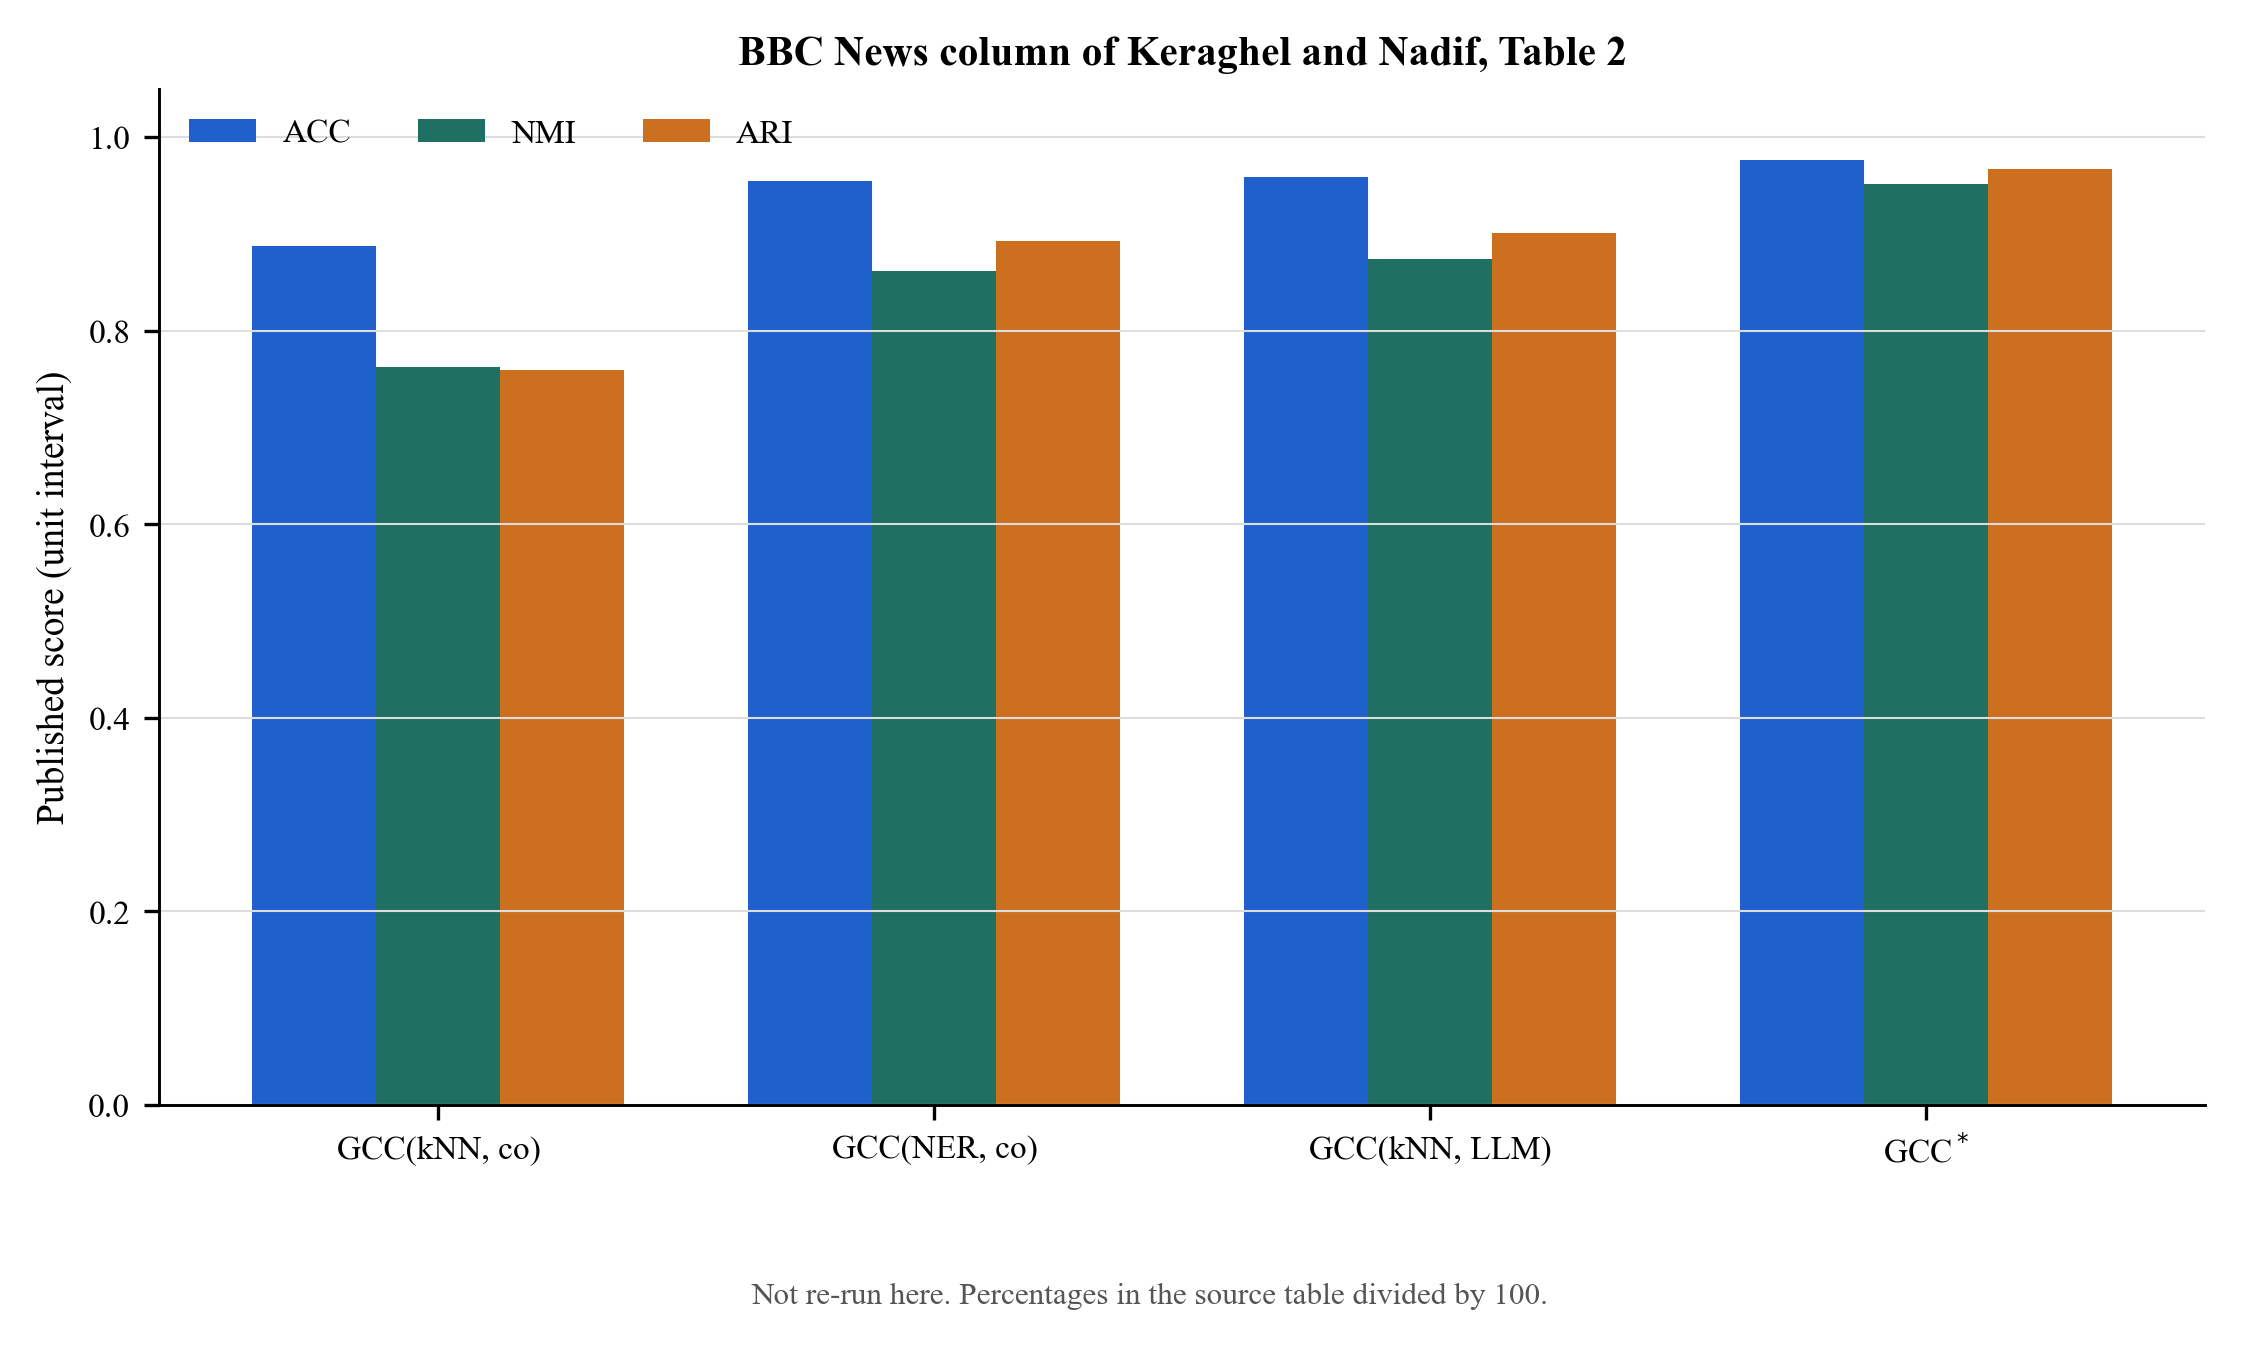
\includegraphics[width=0.88\textwidth]{fig_gcc_published.png}
\caption{BBC News column of Keraghel and Nadif, Table~2,
restated as a grouped bar chart. Not re-run in this
laboratory. Bars start at zero.}
\label{fig:gccpub}
\end{figure}

They also write that $k$-means on LLM embeddings already reaches
about $93\%$ ACC and $91\%$ ARI on BBC in their comparison text,
and that co-occurrence Deep $k$-means collapses on larger packs.
We do not restate their MLSUM, PubMed or ArXiv-10 triples as
our results. Those packs are not scored in
\texttt{experiments/bbc\_final.json}.

Our early lab attempts to copy the spirit of an entity residual
or a thin NER weight on mpnet did not cross $0.9512$. The
\texttt{bbc\_beat\_published.json} file records a best frozen
mix (mpnet+bge+TF-IDF64) at NMI $0.9182$. That is the geometry
ceiling we started from, not the published GCN.

\subsection{Cluster ensembles}

Strehl and Ghosh framed cluster ensembles as knowledge reuse:
several partitions, one consensus~\cite{strehl2002cluster}.
Fred and Jain accumulated co-association evidence across
clusterings~\cite{fred2005eac}. The idea is older than
transformers. If eleven views disagree on a document, the
majority is already a regulariser.

We align every view to a reference mix with the Hungarian
assignment, then take the modal label. Unanimity on this pack
was $1{,}152$ of $2{,}225$ articles in the ensemble run;
disputes on the unique-mode rule were $22$ documents. Majority
NMI $0.9234$ already beats every single view except that it
still sits $0.028$ below GCC$^*$. Spectral $k$NN on the mix
space was a weak voter (NMI $0.6689$ in that same file) and
still sits in the panel because a bad view that is aligned
rarely steals the mode.

Asking a small language model to break those $22$ ties made the
partition worse (panel-on-ties NMI $0.9180$; named desks on
ties $0.9216$). The lesson we kept: do not spend model calls
where the vote is already thin and noisy. Spend them where the
geometry says the document is between two centroids.

\subsection{Language models as clustering guides}

Zhang, Wang and Shang introduced ClusterLLM at EMNLP
2023~\cite{zhang2023clusterllm}. They do not classify named
desks. They ask an instruction-tuned model two kinds of cheap
questions. A hard triplet---does $A$ go with $B$ better than
with $C$---supplies a perspective signal used to fine-tune a
small embedder. Pairwise same-category questions tune
granularity on a hierarchy. They report gains on fourteen
datasets at a mean API cost on the order of sixty cents per
pack. The geometry still lives in the small embedder. The LLM
is a guide.

Huang and He reframe clustering as classification: generate
candidate labels from the pack, merge near-duplicates, then
assign~\cite{huang2024tcllc}. That is the opposite temptation
from ours. Their SIGIR-AP 2025 write-up (preprint
arXiv:2410.00927) argues that in-context labelling removes the
need to fine-tune an embedder. It also names the groups. On
BBC News, naming business, sport, politics, entertainment and
tech would turn the job into zero-shot classification. We
forbid that target in every number placed next to GCC$^*$.

Two failure modes sit between those papers and this draft.
ClusterLLM fine-tunes; we do not. Huang and He generate class
names; we generate one-line event kinds from exemplars and
still assign to unlabeled group indices. Our prompts say
``reply $0$ or $1$'' or ``reply a digit $0$--$4$''. A leak
of the word ``politics'' into an event-kind line is a
prompting defect we report, not a labelled classifier.

\subsection{News corpora and the BBC pack}

Greene and Cunningham released BBC News as a kernel-clustering
example and warned about diagonal dominance~\cite{greene2006bbc}.
The five desks---business, entertainment, politics, sport,
tech---are the gold we score against. Lewis's Reuters
collection~\cite{lewis1997reuters} and Lang's 20 Newsgroups
\cite{lang1995newsweeder} are the usual cousins. Topic Detection
and Tracking~\cite{allan1998tdt} and first-story detection
\cite{petrovic2010fsd} ask a different question (a new event,
not a desk). We ran 20~Newsgroups experiments in the same
repository; those JSON files are listed in
\texttt{bbc\_final.json} and are not the SOTA claim of this
article.

GLUE-style sentence tasks~\cite{wang2018glue} measure
supervised transfer, not clustering NMI. We mention them only
to keep sentence-encoder folklore from being cited as a BBC
desk result.

\subsection{Near-duplicates, linkage, and complaints}

Fellegi and Sunter gave the classical theory of record
linkage~\cite{fellegi1969linkage}. Elmagarmid, Ipeirotis and
Verykios surveyed duplicate detection~\cite{elmagarmid2007duplicate}.
Broder's resemblance sketches sit behind many near-duplicate
pipelines~\cite{broder1997resemblance}. CQADupStack studies
duplicate questions~\cite{hoogeveen2015cqadupstack}. Das and
colleagues clustered civic grievances~\cite{das2020grievance}.
Esperan\c{c}a and colleagues study complaint text in a later
applied paper~\cite{esperanca2025complaint}. Rakhimzhanov,
Belginova and Yedilkhan classify public-transport complaints
with LLMs and embeddings~\cite{rakhimzhanov2025transport}.
Souza, Nogueira and Lotufo released BERTimbau for
Portuguese~\cite{souza2020bertimbau}.

That literature is why CGE production looks the way it does:
TF-IDF, density clustering, a cosine keep-rule. It is also why
a BBC desk stack must not be copied into Ouvidoria by analogy.
Same-event grouping on short Portuguese files is closer to
linkage than to five-way news desks.

Chen and colleagues study intelligent government complaint
platforms in a related applied line~\cite{chen2022igcp}. Silva
and colleagues discuss bridging tools in a later workshop
paper~\cite{silva2026bridging}. We cite them as neighbours in
digital government, not as BBC baselines.

\subsection{Positioning}

Table~\ref{tab:sota-map} is the map we want a reviewer to keep.

\begin{table}[t]
\centering
\caption{Where this laboratory stack sits relative to published
families. Only GCC$^*$ BBC scores and our measured floors are
numeric claims.}
\label{tab:sota-map}
\small
\begin{tabular}{>{\raggedright\arraybackslash}p{0.28\textwidth}
                >{\raggedright\arraybackslash}p{0.30\textwidth}
                >{\raggedright\arraybackslash}p{0.32\textwidth}}
\toprule
Family & Typical move & Relation to this draft \\
\midrule
Lexical + density
  & TF-IDF, DBSCAN, HDBSCAN
  & CGE production; not the BBC claim \\
Frozen embedder + $k$-means
  & SBERT / MPNet / BGE
  & Our geometry; ceiling $\approx 0.92$ NMI \\
Joint deep clustering
  & DEC, GCC
  & GCC$^*$ is the published BBC mark \\
Cluster ensembles
  & Strehl, Fred \& Jain
  & Our majority of 11 \\
LLM as embedder guide
  & ClusterLLM triplets
  & Same spirit, no fine-tune here \\
LLM as label generator
  & Huang \& He
  & Forbidden as the GCC$^*$ comparator \\
Gated LLM audit
  & this draft
  & Model sees exemplars, not desk names \\
\bottomrule
\end{tabular}
\end{table}

The honest sentence is short. GCC$^*$ trains a graph model.
ClusterLLM fine-tunes a small embedder with triplet feedback.
Huang and He name classes. We freeze the embedders, vote, and
let Claude read a gated rim. The published number we have to
beat is still Table~\ref{tab:gcc-published}, last row.

%% ====================================================================
\section{Problem, corpus, and protocol}
%% ====================================================================

\subsection{Task}

Let $D=\{d_1,\ldots,d_N\}$ be the BBC News articles,
$N=2{,}225$. Gold desks $y_i\in\{1,\ldots,5\}$ exist for
scoring and are unused when a gate chooses an index set
$S\subset\{1,\ldots,N\}$. A method returns a partition
$\hat{y}\in\{1,\ldots,5\}^N$. We report
\[
\mathrm{NMI}(\hat{y},y),\qquad
\mathrm{ARI}(\hat{y},y),\qquad
\mathrm{ACC}(\hat{y},y)
\]
with NMI the arithmetic-average sklearn form~\cite{vinh2010nmi}
and ACC after Hungarian alignment~\cite{kuhn1955hungarian}.

\subsection{Fair versus probe}

A run is \emph{fair} if $S$ is a function of $\hat{y}$ and the
embedding geometry only. Pair prompts show two exemplar lists
and ask for $0$ or $1$. Five-way prompts show five exemplar
lists and ask for a digit. No desk string is the legal answer.

A run is a \emph{probe} if gold intersects $S$ (for example
``the 21 majority-border errors''). Probes diagnose. They do
not sit on the GCC$^*$ line.

The oracle that flips every majority error inside a margin
band uses gold as the flip. The $n=80$ oracle in
\texttt{bbc\_nmi\_lift.json} reaches NMI $0.9527$. That is a
ceiling, not a method.

\subsection{Why $k=5$ is given}

GCC$^*$ discusses reading $k$ from a dendrogram after
over-segmentation. We do not claim an automatic $k$. BBC News
is distributed as five desks. The comparison is on that $k$.
A production complaint system does not get $k$ from Greene and
Cunningham.

\subsection{Randomness and devices}

Cluster seeds use $\mathrm{RNG}=20260925$ as in the experiment
scripts. Sentence embeddings were computed on CPU after an MPS
hang on this machine. Spectral clustering on the mix space
moved majority NMI by a few points on one early run
($0.9221$ versus $0.9234$); the kept majority labels are the
$0.9234$ snapshot stored as stage~1 in the floor table.

%% ====================================================================
\section{Method}
%% ====================================================================

The stack has two blocks. Block~A is unsupervised and cheap.
Block~B is a gated audit. Figure~\ref{fig:pipeline} is the
protocol. Figure~\ref{fig:gates} shows what the model is
allowed to see. Figure~\ref{fig:stairs} is the measured NMI
of the kept path. All numbers come from
\texttt{experiments/bbc\_final.json} unless a caption says
otherwise.

\subsection{Block A: eleven views and a majority}

Let $Z_{\mathrm{mp}}$ and $Z_{\mathrm{bge}}$ be L2-normalised
document matrices from the cached MPNet and BGE encoders.
Let $T$ be a 64-dimensional TF-IDF SVD slice. The mix space
used for margins and neighbours is
\[
Z=\mathrm{normalize}\bigl([Z_{\mathrm{mp}}\,|\,Z_{\mathrm{bge}}\,|\,0.20\,T]\bigr).
\]
Title and chunk views reuse MPNet on titles and on mean-pooled
chunks. The eleven partitions are:

\begin{enumerate}
\item $k$-means on $Z_{\mathrm{mp}}$;
\item $k$-means on $Z_{\mathrm{bge}}$;
\item $k$-means on the concatenation of the two encoders;
\item $k$-means on $Z$ (the mix);
\item $k$-means on MPNet concatenated with a $0.25$ TF-IDF slice;
\item $k$-means on chunk-mean MPNet;
\item $k$-means on MPNet concatenated with a $0.15$ title vector;
\item factorial $k$-means on $Z$;
\item a three-matrix consensus on $(Z_{\mathrm{mp}},Z_{\mathrm{bge}},T)$;
\item a diagonal Gaussian mixture on $Z$;
\item spectral clustering, $k$NN affinity, $25$ neighbours, on $Z$.
\end{enumerate}

Each partition other than the mix is Hungarian-aligned to the
mix labels~\cite{kuhn1955hungarian}. The majority label is the
mode of the eleven aligned votes. Table~\ref{tab:panel} lists
the single-view scores from
\texttt{experiments/bbc\_llm\_ensemble.json}. Majority NMI
$0.9234$ is higher than the best single view ($0.9182$).
Figure~\ref{fig:panel} is the same panel as a bar chart.

\begin{figure}[t]
\centering
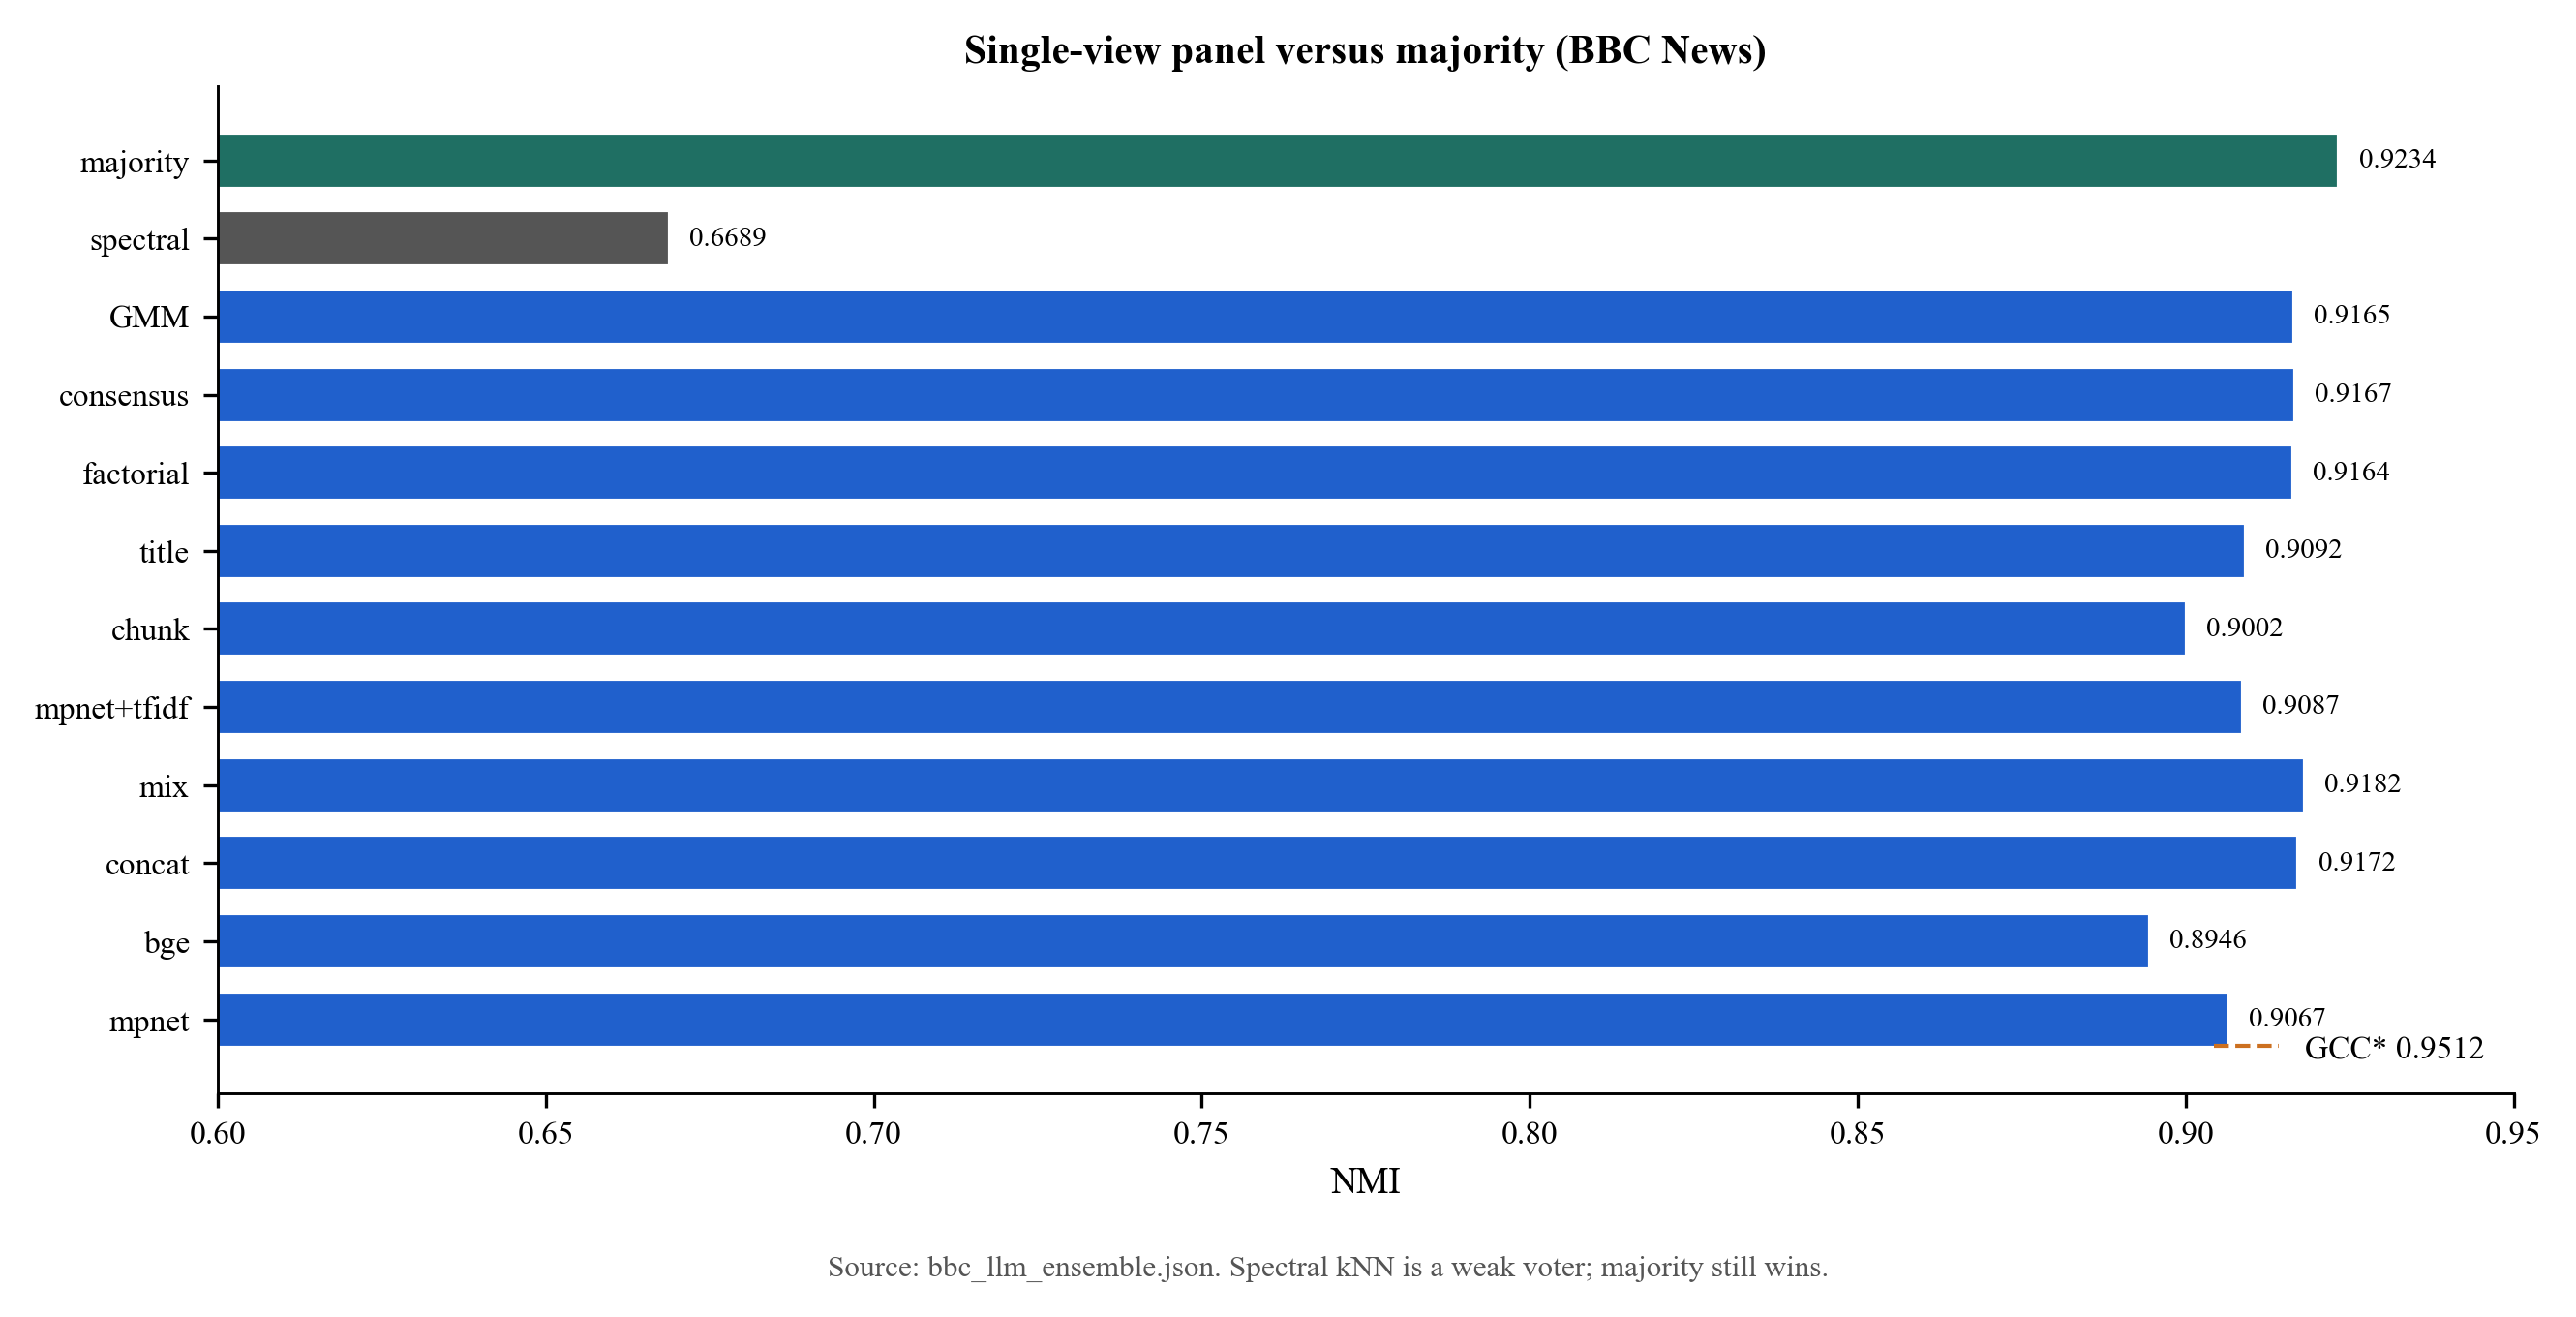
\includegraphics[width=0.92\textwidth]{fig_panel.png}
\caption{Single-view NMI versus the aligned majority.
Dashed line: published GCC$^*$ ($0.9512$). Source:
\texttt{bbc\_llm\_ensemble.json}.}
\label{fig:panel}
\end{figure}

\begin{table}[t]
\centering
\caption{Single-view panel on BBC News, then majority.
Source: \texttt{bbc\_llm\_ensemble.json}. Measured.}
\label{tab:panel}
\small
\begin{tabular}{lccc}
\toprule
View & NMI & ARI & ACC \\
\midrule
mpnet $k$-means & 0.9067 & 0.9306 & 0.9708 \\
bge $k$-means & 0.8946 & 0.9197 & 0.9667 \\
concat mpnet+bge & 0.9172 & 0.9401 & 0.9748 \\
mix (mpnet+bge+$0.20$ TF-IDF64) & 0.9182 & 0.9412 & 0.9753 \\
mpnet+TF-IDF & 0.9087 & 0.9309 & 0.9708 \\
chunk-mean & 0.9002 & 0.9263 & 0.9690 \\
title mix & 0.9092 & 0.9329 & 0.9717 \\
factorial mix & 0.9164 & 0.9393 & 0.9744 \\
consensus of three matrices & 0.9167 & 0.9387 & 0.9748 \\
diagonal GMM on mix & 0.9165 & 0.9402 & 0.9748 \\
spectral $k$NN on mix & 0.6689 & 0.5081 & 0.5384 \\
\midrule
majority of 11 (aligned) & 0.9234 & 0.9451 & 0.9771 \\
\bottomrule
\end{tabular}
\end{table}

Centroid $c_g$ of group $g$ is the mean of $Z$ rows with that
majority label, renormalised. The margin of document $i$ is
the gap between cosine to its assigned centroid and cosine to
the next nearest centroid. Thin margin means small gap.

\subsection{Block B: gated audit}

Models are \texttt{claude-sonnet-4-6} (first reader) and
\texttt{claude-opus-4-6} (second reader). Calls are cached.
Workers~$=4$. The assigner never receives the five desk
strings as the legal output vocabulary.

\subsubsection{Floor 2 --- pair on the thinnest 80}

Sort documents by increasing margin. Take $80$. For each,
show two exemplar lists from the two nearest groups. Sonnet
answers $0$ or $1$. A five-way read fires only if that bit
leaves the pair. This single gate lifted NMI from $0.9234$
to $0.9358$ (41 errors). A five-way-only border of 80 or 120
was worse than the pair rule in
\texttt{bbc\_nmi\_lift.json}.

\subsubsection{Floor 3 --- Opus on flips and close-3}

Documents whose pair decision flipped, plus documents whose
second and third centroids differ by less than $0.02$ in
cosine, go to Opus with five exemplar blocks. NMI $0.9381$,
39 errors.

\subsubsection{Floor 4 --- odd-one-out}

Sonnet answers whether the article belongs with its current
exemplars. A ``no'' goes to Opus. NMI $0.9430$, 36 errors.

\subsubsection{Floor 5 --- neighbour revolt}

If at least four of seven cosine neighbours in $Z$ carry
another majority label, Opus rereads. NMI $0.9466$, 34
errors. Figure~\ref{fig:gates} is this family of tests.

\subsubsection{Floor 7 --- foreign neighbour}

If the nearest neighbour in another cluster is closer than
the second neighbour in the assigned cluster, Opus rereads.
NMI $0.9482$, 33 errors. One fix, zero breaks in the
recorded step.

\subsubsection{Floor 12 --- rim exemplars}

Exemplars are taken from the rim of the closest centroid
pair rather than from the core. NMI $0.9487$. Same error
count, slightly kinder pairwise scores.

\subsubsection{Floor 14 --- event kind}

Each group receives a one-line event kind written from its
own exemplars, with an instruction not to use newspaper
section names. Sonnet then matches the article to the kind
of event, not the industry of a company in the title. Opus
confirms flips. NMI $0.9496$, 31 errors (5 fix, 3 broke).
The recorded blurbs still drifted toward desk language
(``entertainment and arts'', ``UK political news''). The
assigner output remains an index. We report the leak
instead of pretending the prompt stayed clean.

\subsubsection{Floor 15 --- closest-pair keep}

Let $S=C^\top C$ on the five centroids. The closest pair on
this run was groups $\{2,3\}$ in the majority index (the
business-facing and digital-facing piles in the aligned
geometry). A Floor~14 flip is kept only if both the old and
new labels sit in that pair. Off-pair flips---a game review
leaving the digital group---are dropped. Measured NMI
$0.9520$, ARI $0.9673$, ACC $0.9865$, 30 errors (4 fix, 1
broke). This is the number we place next to GCC$^*$.

\subsection{Discarded gates}

Table~\ref{tab:discarded} lists gates that were implemented
and not kept. Remargin after a move broke a correct article
and fixed none. TF-IDF disagreement with the majority fixed
two and broke three. The second-closest centroid pair
(politics--business in that run) broke one. Re-running
revolt after labels moved found no new members. Closest-pair
routing with stale exemplars was a no-op.

\begin{table}[t]
\centering
\caption{Discarded floors. Source: \texttt{bbc\_final.json}.
Measured. Not in the final partition.}
\label{tab:discarded}
\small
\begin{tabular}{llp{0.42\textwidth}c}
\toprule
Floor & Why dropped & NMI after \\
\midrule
6a/6b & no new revolt after moves & 0.9466 \\
8 & remargin pair broke 1, fixed 0 & 0.9456 \\
9 & tight foreign on remargin: no lift & 0.9456 \\
10 & TF-IDF disagree 2 fix / 3 broke & 0.9472 \\
11 & closest pair, old exemplars, $0/0$ & 0.9482 \\
13 & second pair (politics--business) broke 1 & 0.9476 \\
\bottomrule
\end{tabular}
\end{table}

\subsection{What we refuse to call clustering}

Named-desk prompts on the border are zero-shot
classification. Gold-picked border errors (NMI $0.9468$ in
\texttt{bbc\_claude\_border\_errors.json}) use the label file
as a sampler. Both are in the JSON trail. Neither is the
headline number.

%% ====================================================================
\section{Experimental setup}
%% ====================================================================

\subsection{Data}

BBC News follows Greene and Cunningham~\cite{greene2006bbc}.
Texts and gold desks are loaded by
\texttt{experiments/run\_public\_benchmarks.py}. Titles and
ledes are the first line and a clipped lead for prompts.

\subsection{Software}

Python, NumPy, scikit-learn~\cite{pedregosa2011sklearn}.
Anthropic Messages API, models named above. Caches live under
\texttt{experiments/data/} and are gitignored. Label arrays
for kept floors are stored under
\texttt{experiments/results/bbc\_labels/}.

\subsection{Scoring script}

\texttt{experiments/run\_bbc\_final\_score.py} reloads stage
labels and writes \texttt{bbc\_final\_scores.json}. The
headline triple is taken from Floor~15 in
\texttt{bbc\_final.json}.

\subsection{What we did not tune on gold}

We did not grid-search prompt wording against NMI. We did
not add a document to a gate because it was a known error.
When a gate looked promising we applied it to a geometry
set, scored once, and kept or discarded on the net fix/break
count.

%% ====================================================================
\section{Results}
%% ====================================================================

\subsection{Kept staircase}

Table~\ref{tab:floors} is the kept path. Figure~\ref{fig:stairs}
plots NMI against the published dashed line.

\begin{table}[t]
\centering
\caption{Kept floors on BBC News. Source:
\texttt{experiments/bbc\_final.json}. Gold does not pick
documents.}
\label{tab:floors}
\small
\begin{tabular}{rlrrrr}
\toprule
Floor & Gate & NMI & ARI & ACC & Err. \\
\midrule
1 & Majority of 11 & 0.9234 & 0.9451 & 0.9771 & 51 \\
2 & Sonnet pair on thin 80 & 0.9358 & 0.9554 & 0.9816 & 41 \\
3 & Opus on flips and close-3 & 0.9381 & 0.9575 & 0.9825 & 39 \\
4 & Odd-one-out then Opus & 0.9430 & 0.9607 & 0.9838 & 36 \\
5 & Neighbour revolt $4/7$ & 0.9466 & 0.9628 & 0.9847 & 34 \\
7 & Foreign neighbour then Opus & 0.9482 & 0.9640 & 0.9852 & 33 \\
12 & Rim exemplars, closest pair & 0.9487 & 0.9639 & 0.9852 & 33 \\
14 & Event-kind pair then Opus & 0.9496 & 0.9663 & 0.9861 & 31 \\
15 & Keep closest-pair flips only & \textbf{0.9520} & \textbf{0.9673} & \textbf{0.9865} & 30 \\
\midrule
--- & GCC$^*$ published & 0.9512 & 0.9666 & 0.9761 & --- \\
\bottomrule
\end{tabular}
\end{table}

\begin{figure}[t]
\centering
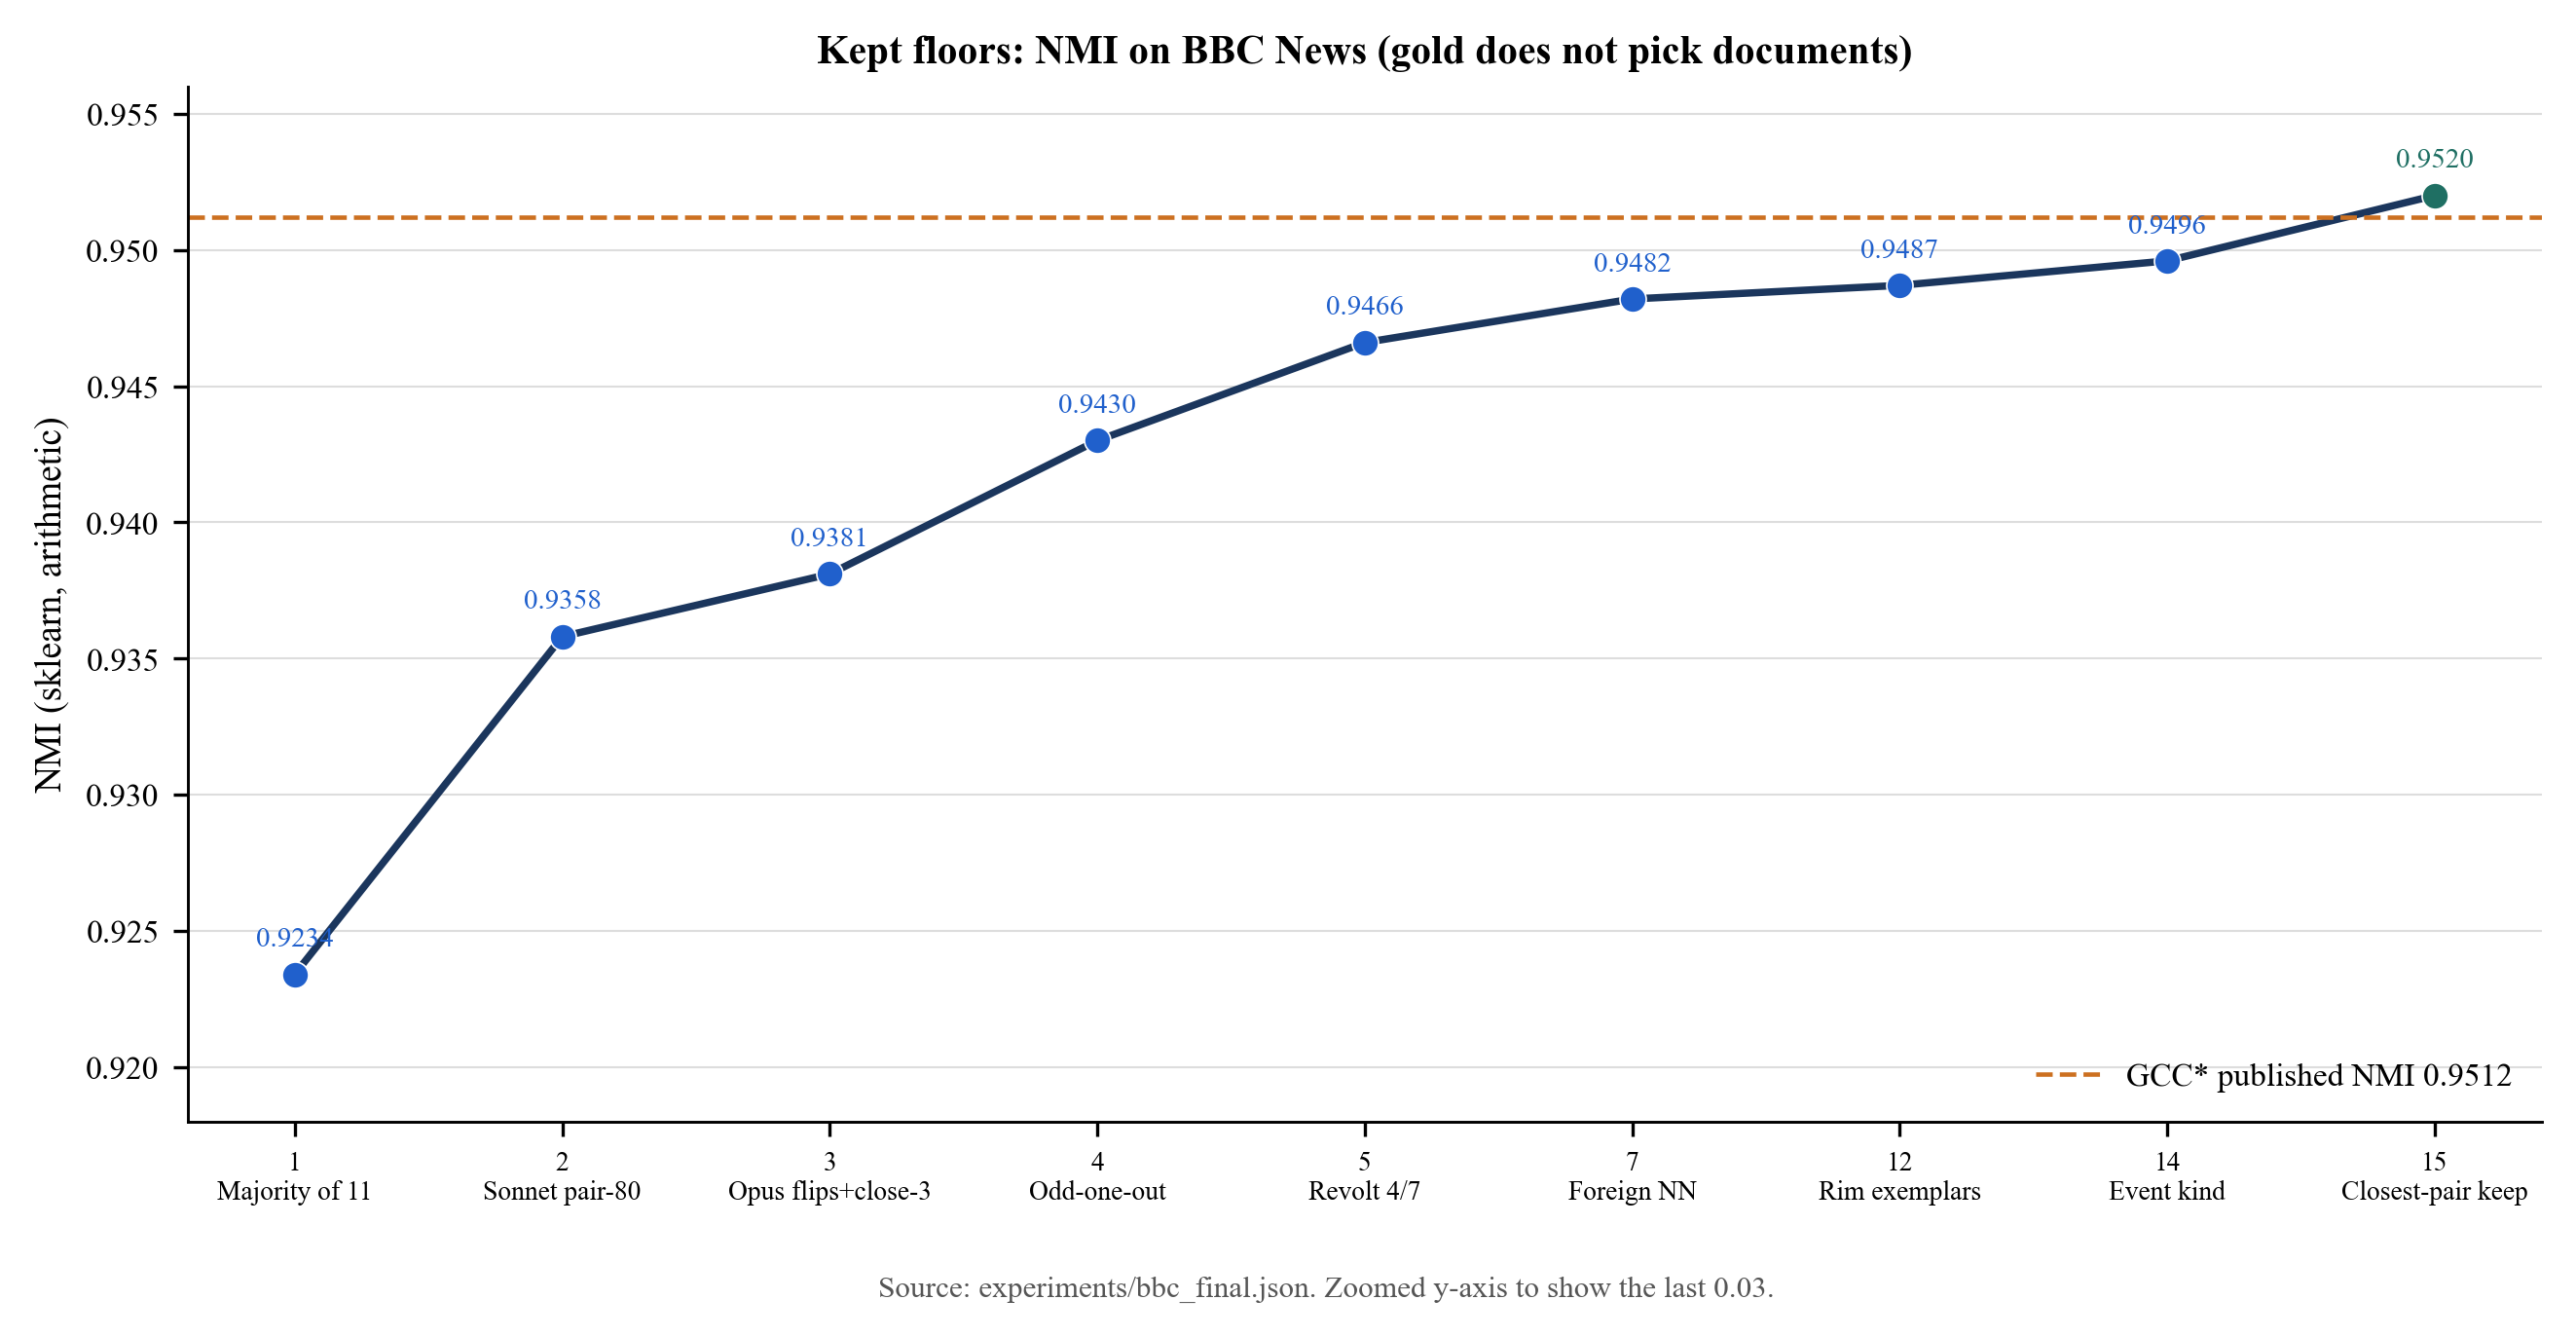
\includegraphics[width=0.94\textwidth]{fig_nmi_staircase.png}
\caption{Measured NMI on the kept floors. Dashed line:
published GCC$^*$ ($0.9512$). Laboratory only. CGE production
unchanged.}
\label{fig:stairs}
\end{figure}

Accuracy crossed the published $0.9761$ already at Floor~1
($0.9771$). NMI lagged until the event-kind gate and the
keep rule. That lag is the business--tech--politics leak:
Hungarian ACC can look fine while NMI still feels the
swap of a few dozen articles between large desks.

\subsection{Probes that must not be compared to GCC$^*$}

\begin{table}[t]
\centering
\caption{Probes. Gold takes part in the set or the flip.
Not comparable to Table~\ref{tab:gcc-published}.}
\label{tab:probes}
\small
\begin{tabular}{lccc}
\toprule
Probe & NMI & ARI & ACC \\
\midrule
Sonnet pair on gold-picked 21 border errors & 0.9468 & 0.9631 & 0.9847 \\
Oracle flip of 21 thinnest-margin majority errors & 0.9527 & 0.9674 & 0.9865 \\
Oracle majority-border $n=120$ & 0.9609 & 0.9737 & 0.9892 \\
\bottomrule
\end{tabular}
\end{table}

The gold-picked pair sits \emph{below} the fair Floor~15. Using
gold as a sampler made a worse headline than refusing it.
The $n=80$ oracle sits $0.0007$ above Floor~15: three leftover
flips in that band would have been enough, and the keep rule
found a different three.

\subsection{Leftovers}

Floor~15 leaves 30 disagreements with gold. The working note
in the architecture scripts is that most remaining leaks are
gold-business articles sitting in the digital or parliament
piles: telecom appointments, pensions, the chancellor, brand
names that embeddings treat as products. We do not publish a
full title list in this draft. The label array
\texttt{bbc\_stage15\_labels.npy} is the artefact to audit.

\subsection{Academic figures of the kept path}

Figure~\ref{fig:pipeline} is the protocol. Figure~\ref{fig:compare}
places Floor~1, Floor~15 and published GCC$^*$ on the same
three metrics. Figure~\ref{fig:errors} counts leftover
errors. Figure~\ref{fig:protocol} separates the fair
headline from gold-using probes. Figure~\ref{fig:leak} is
the qualitative residual (brand versus event), not a
confusion cell.

\begin{figure}[t]
\centering
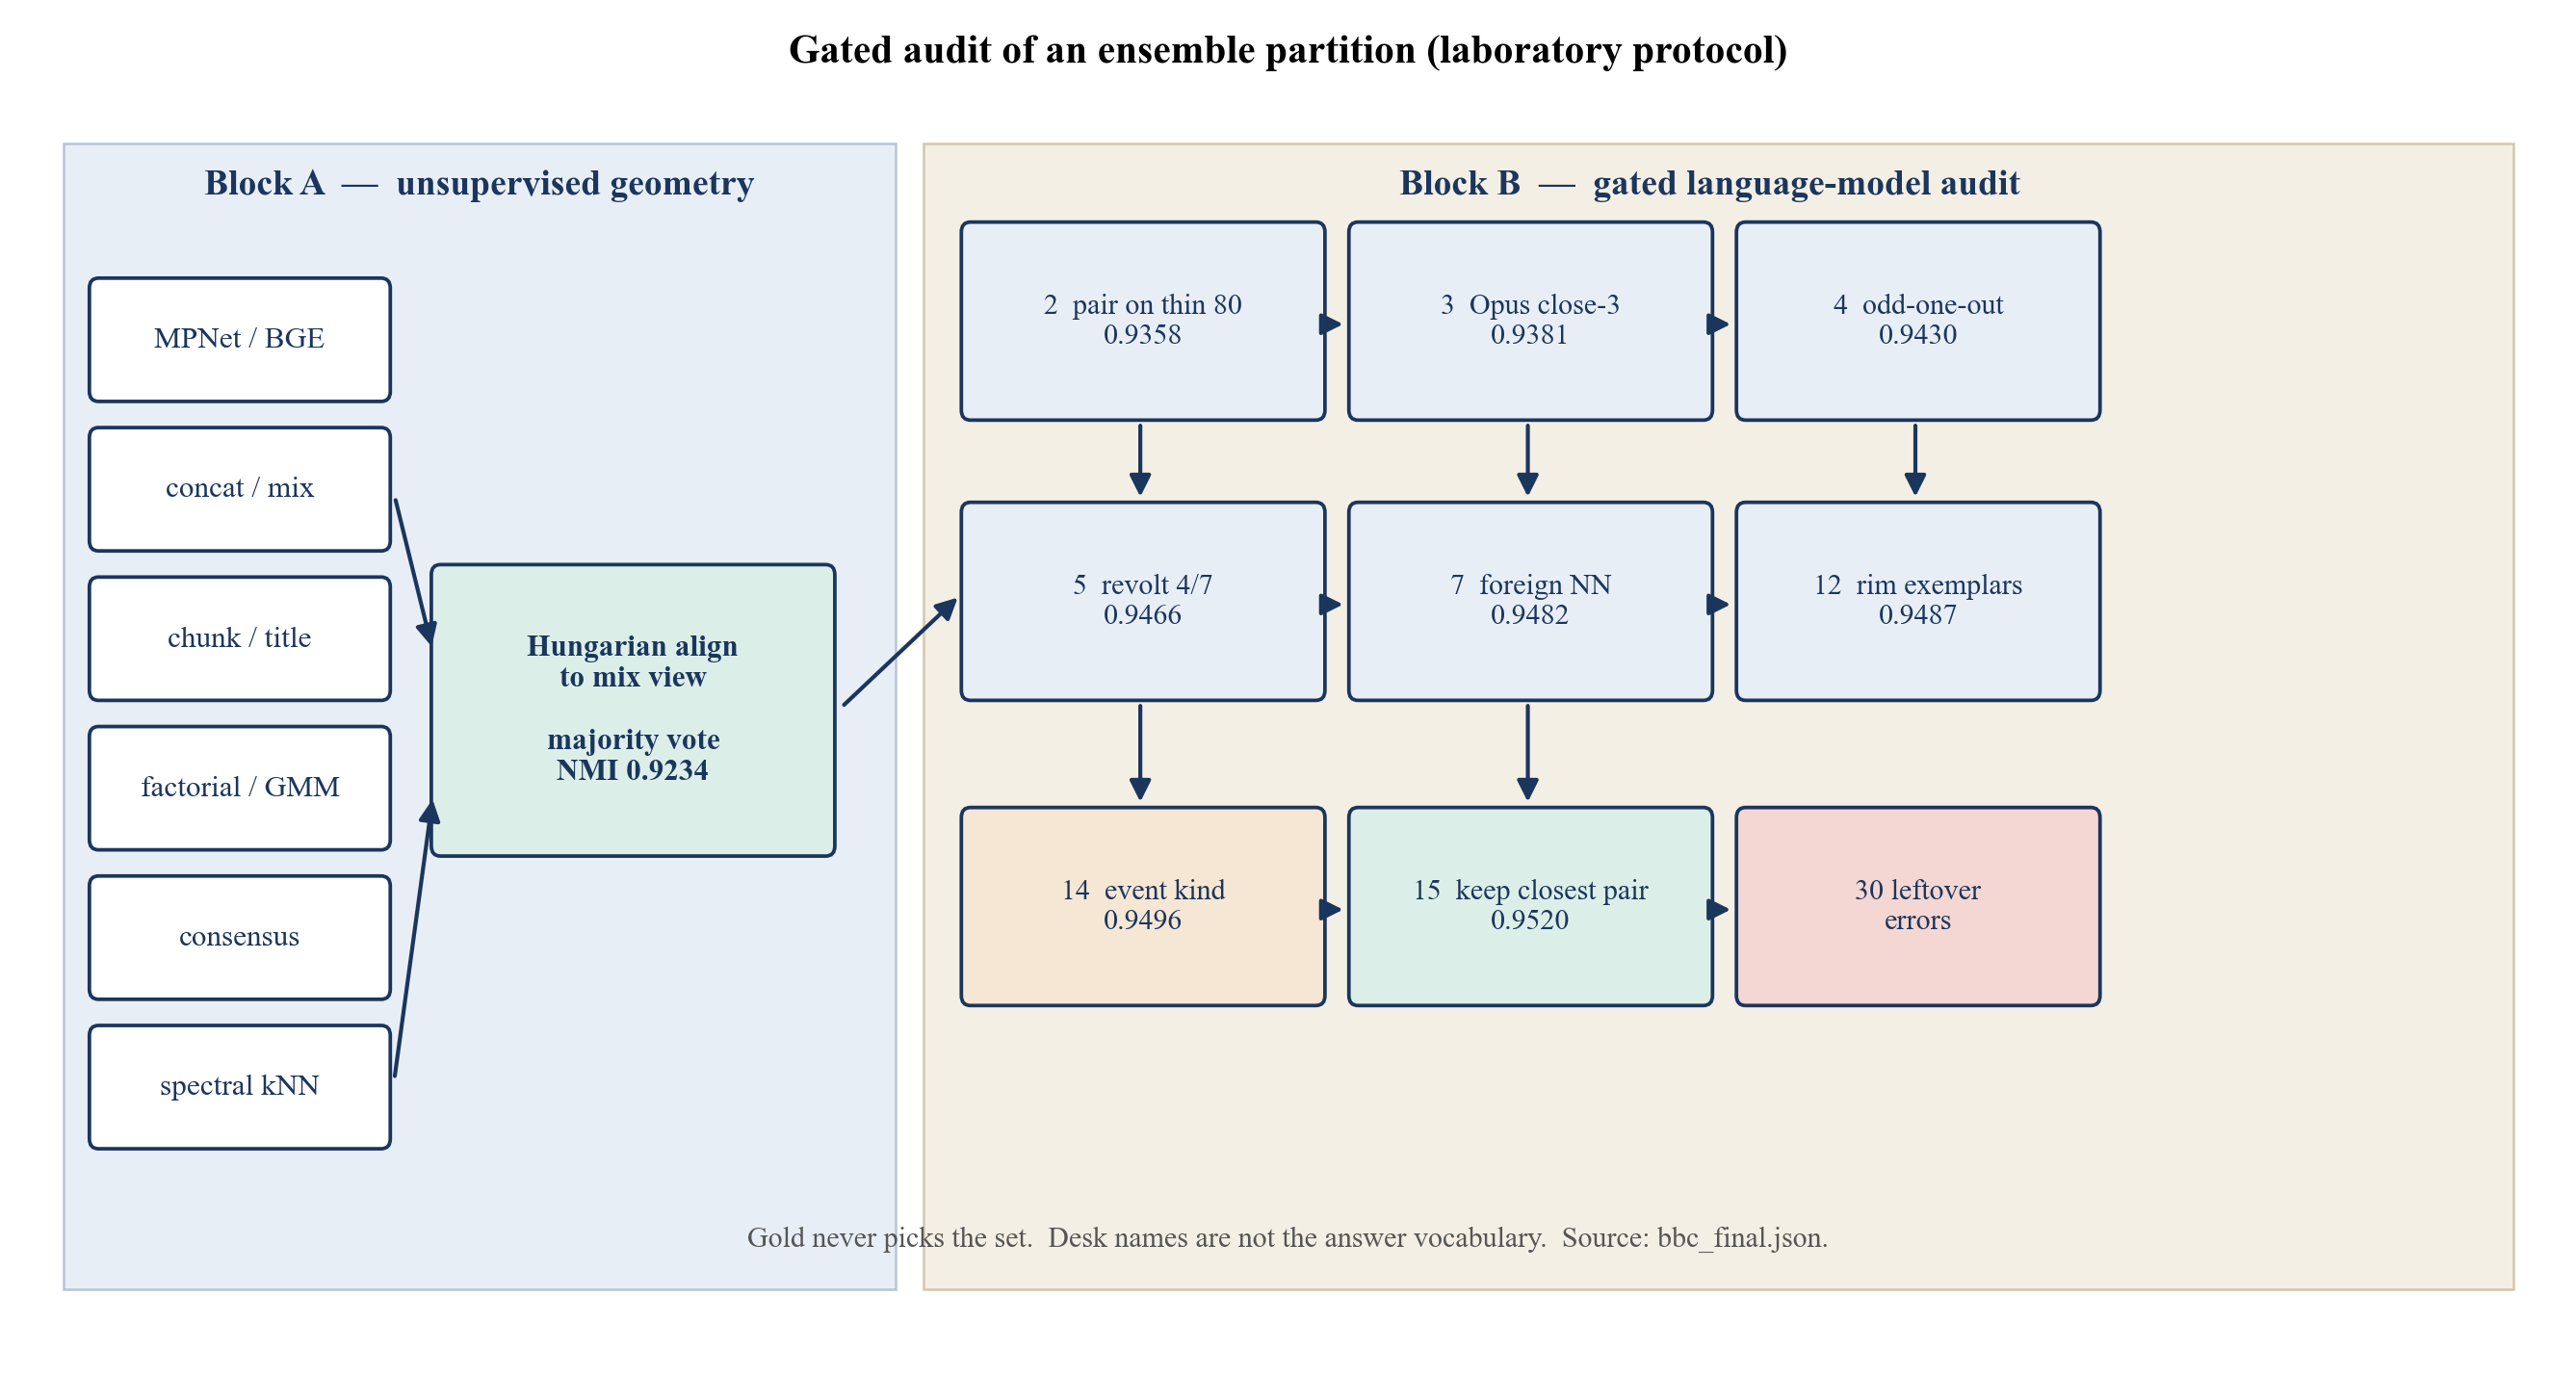
\includegraphics[width=0.96\textwidth]{fig_pipeline.png}
\caption{Laboratory protocol. Block~A is an aligned majority
of eleven clusterings. Block~B is a gated audit. NMI values
are measured (\texttt{bbc\_final.json}).}
\label{fig:pipeline}
\end{figure}

\begin{figure}[t]
\centering
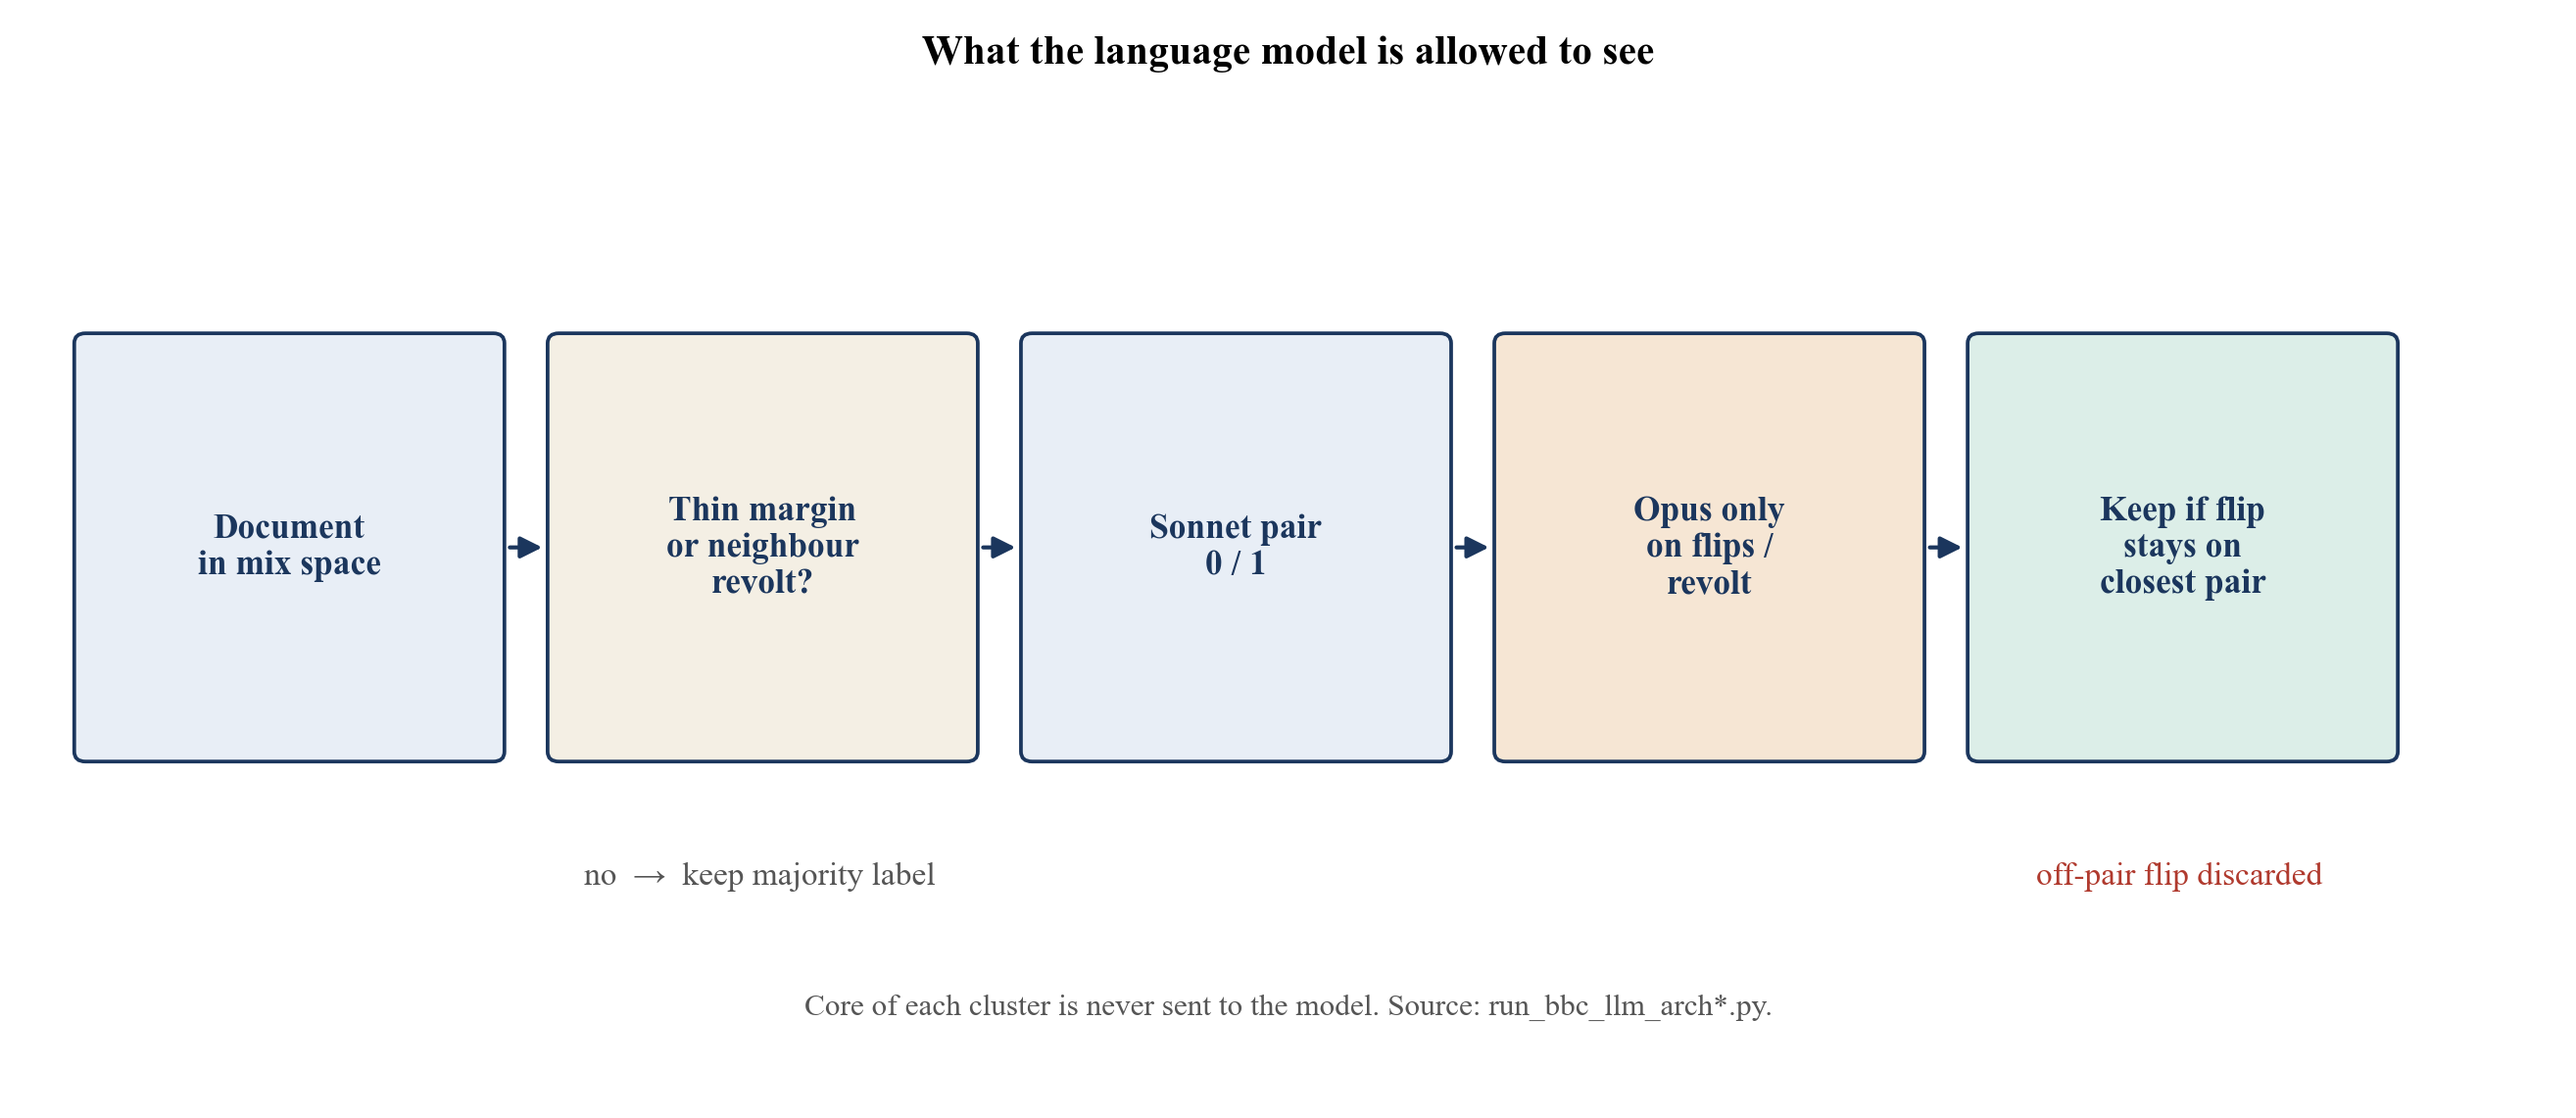
\includegraphics[width=0.94\textwidth]{fig_gates.png}
\caption{The language model sees a document only when a
geometry gate fires. Off-pair flips are discarded at
Floor~15.}
\label{fig:gates}
\end{figure}

\begin{figure}[t]
\centering
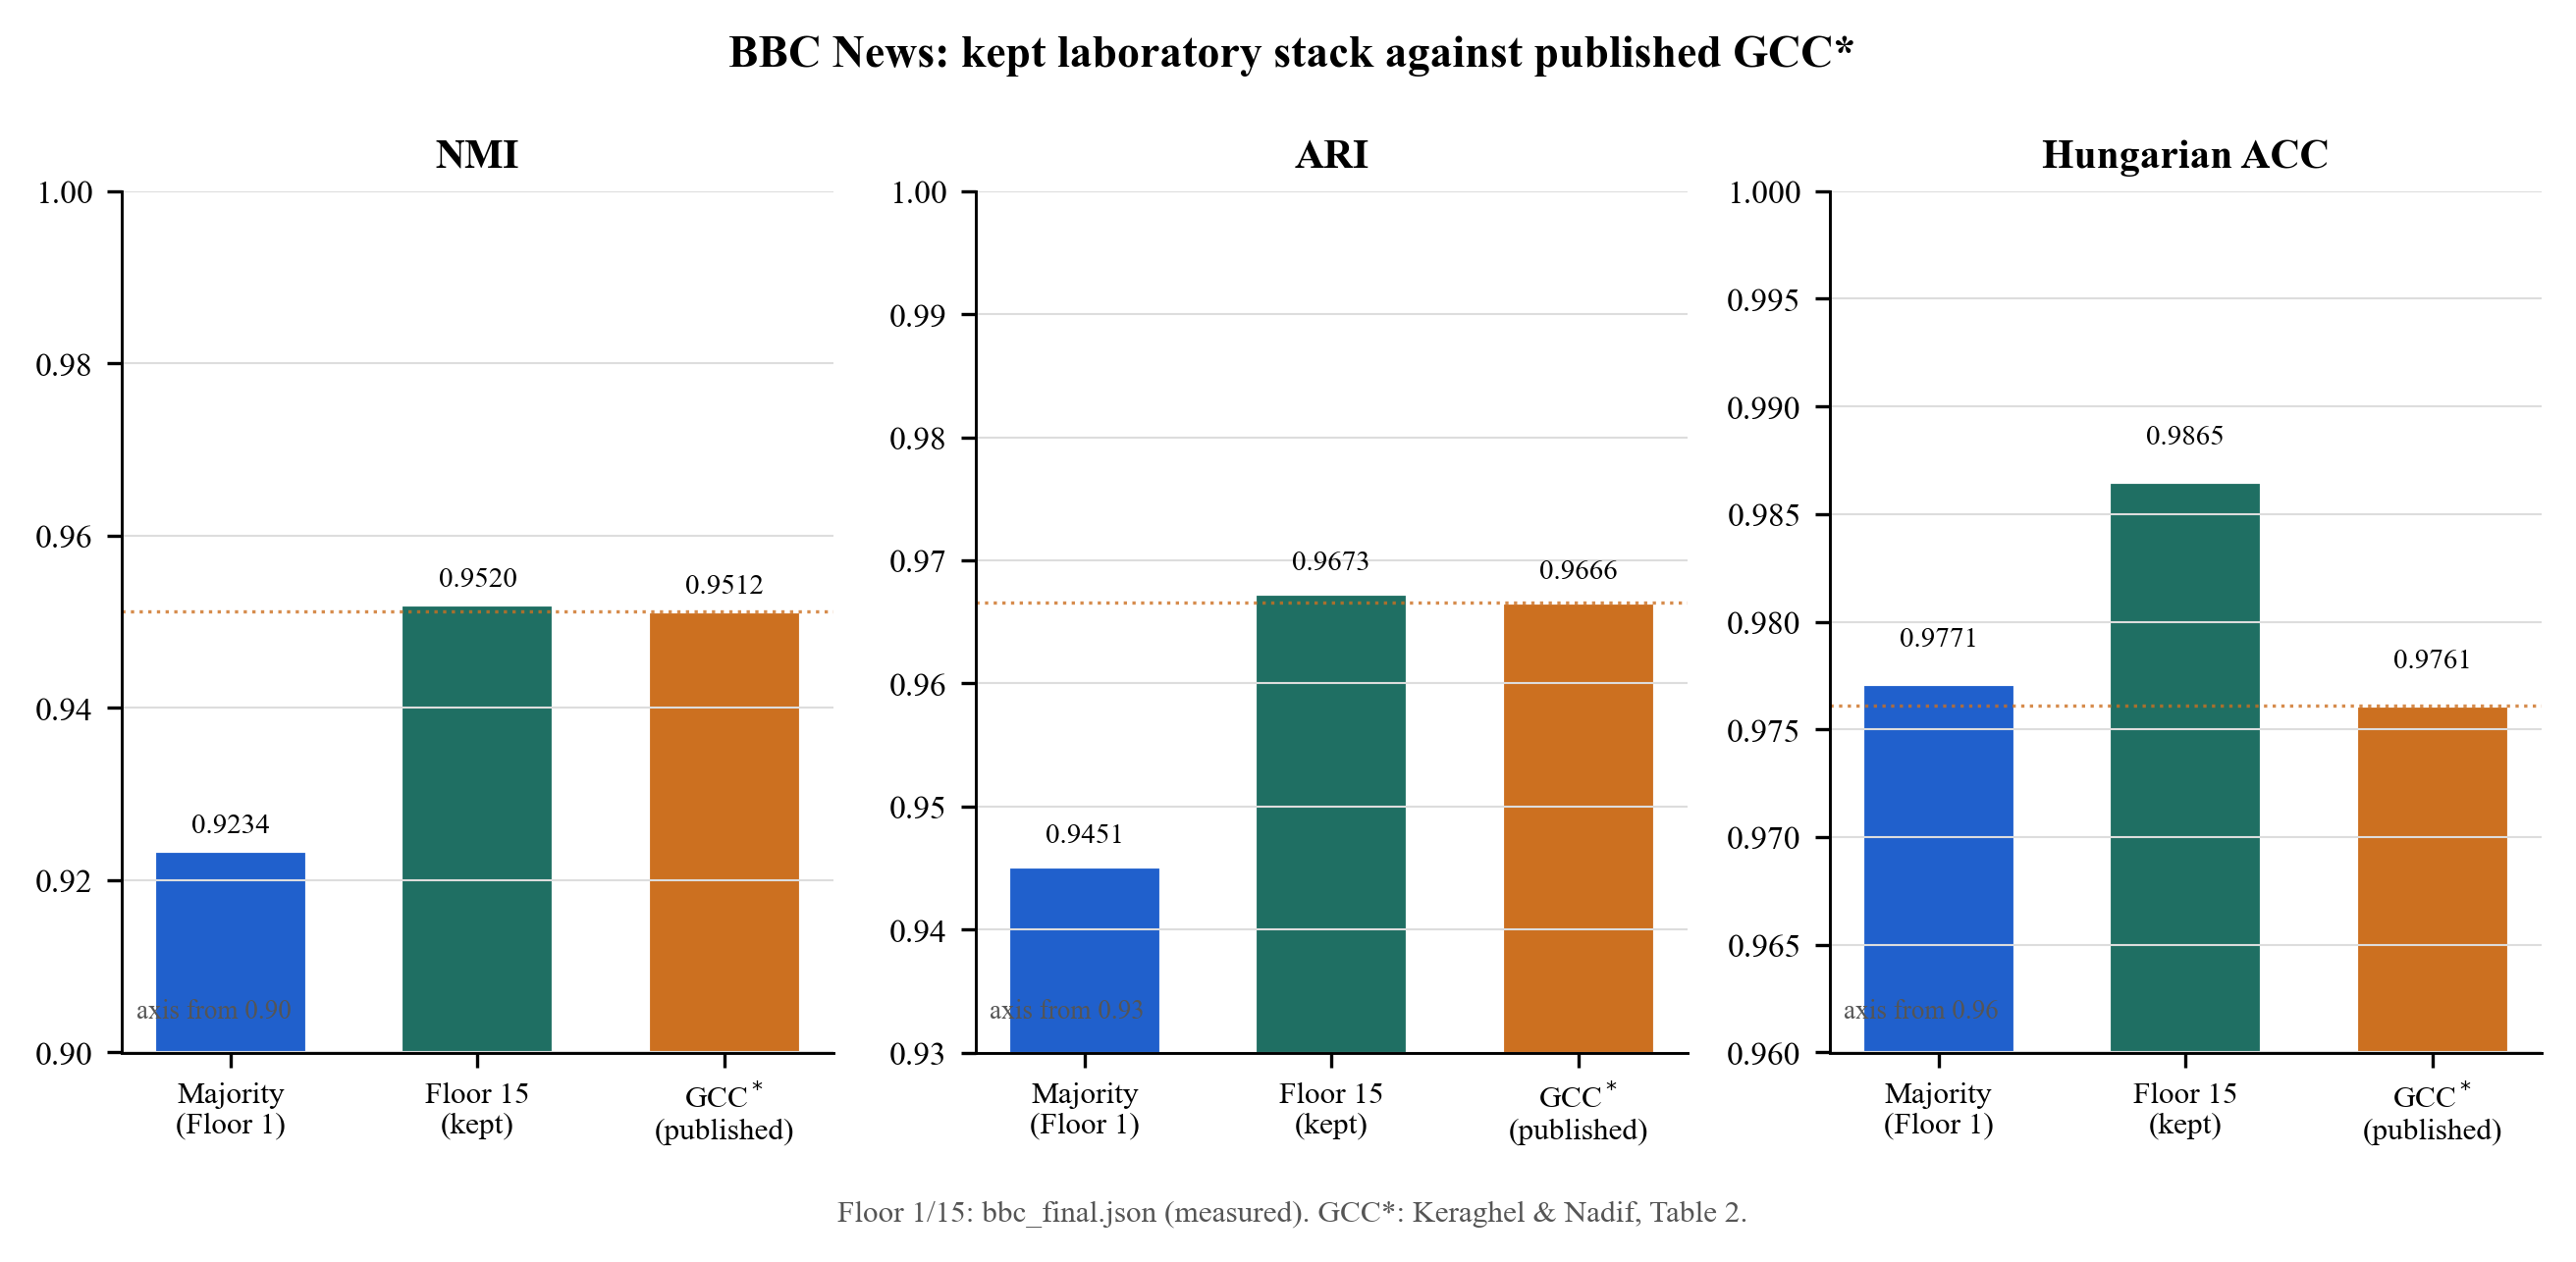
\includegraphics[width=0.94\textwidth]{fig_metrics_compare.png}
\caption{Kept stack against published GCC$^*$ on NMI, ARI
and Hungarian accuracy. Each panel states its $y$ minimum;
the zoom is for the last few points, not a zero-baseline
bar.}
\label{fig:compare}
\end{figure}

\begin{figure}[t]
\centering
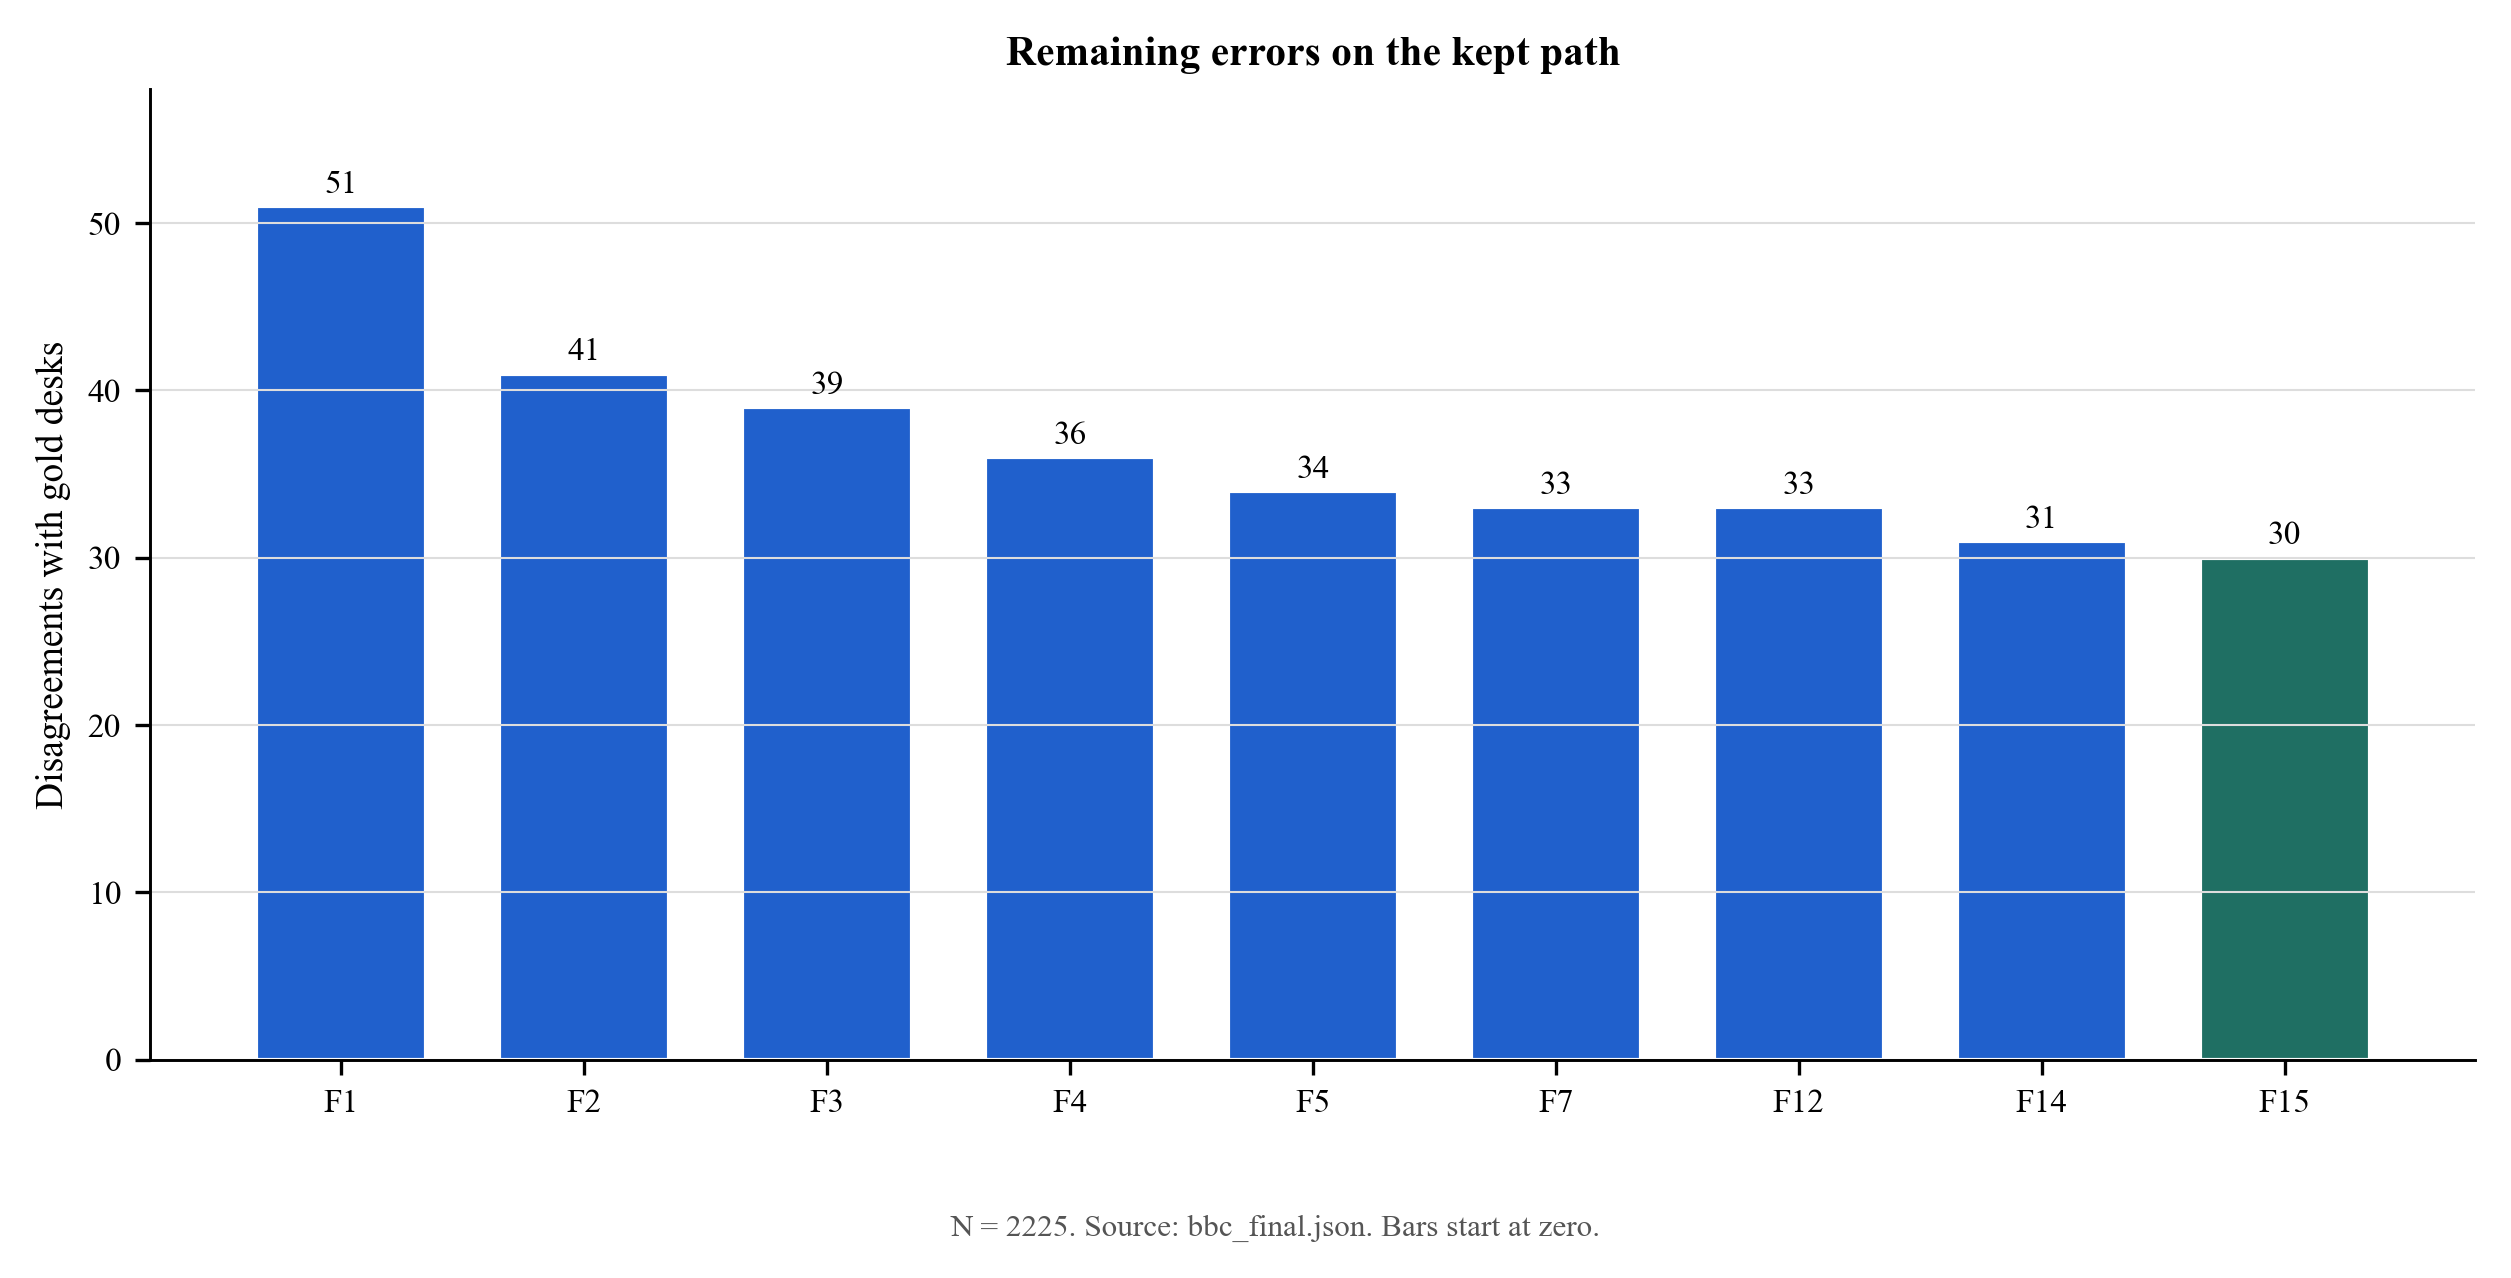
\includegraphics[width=0.92\textwidth]{fig_errors.png}
\caption{Remaining disagreements with gold desks on the kept
path. Bars start at zero. $N=2{,}225$.}
\label{fig:errors}
\end{figure}

\begin{figure}[t]
\centering
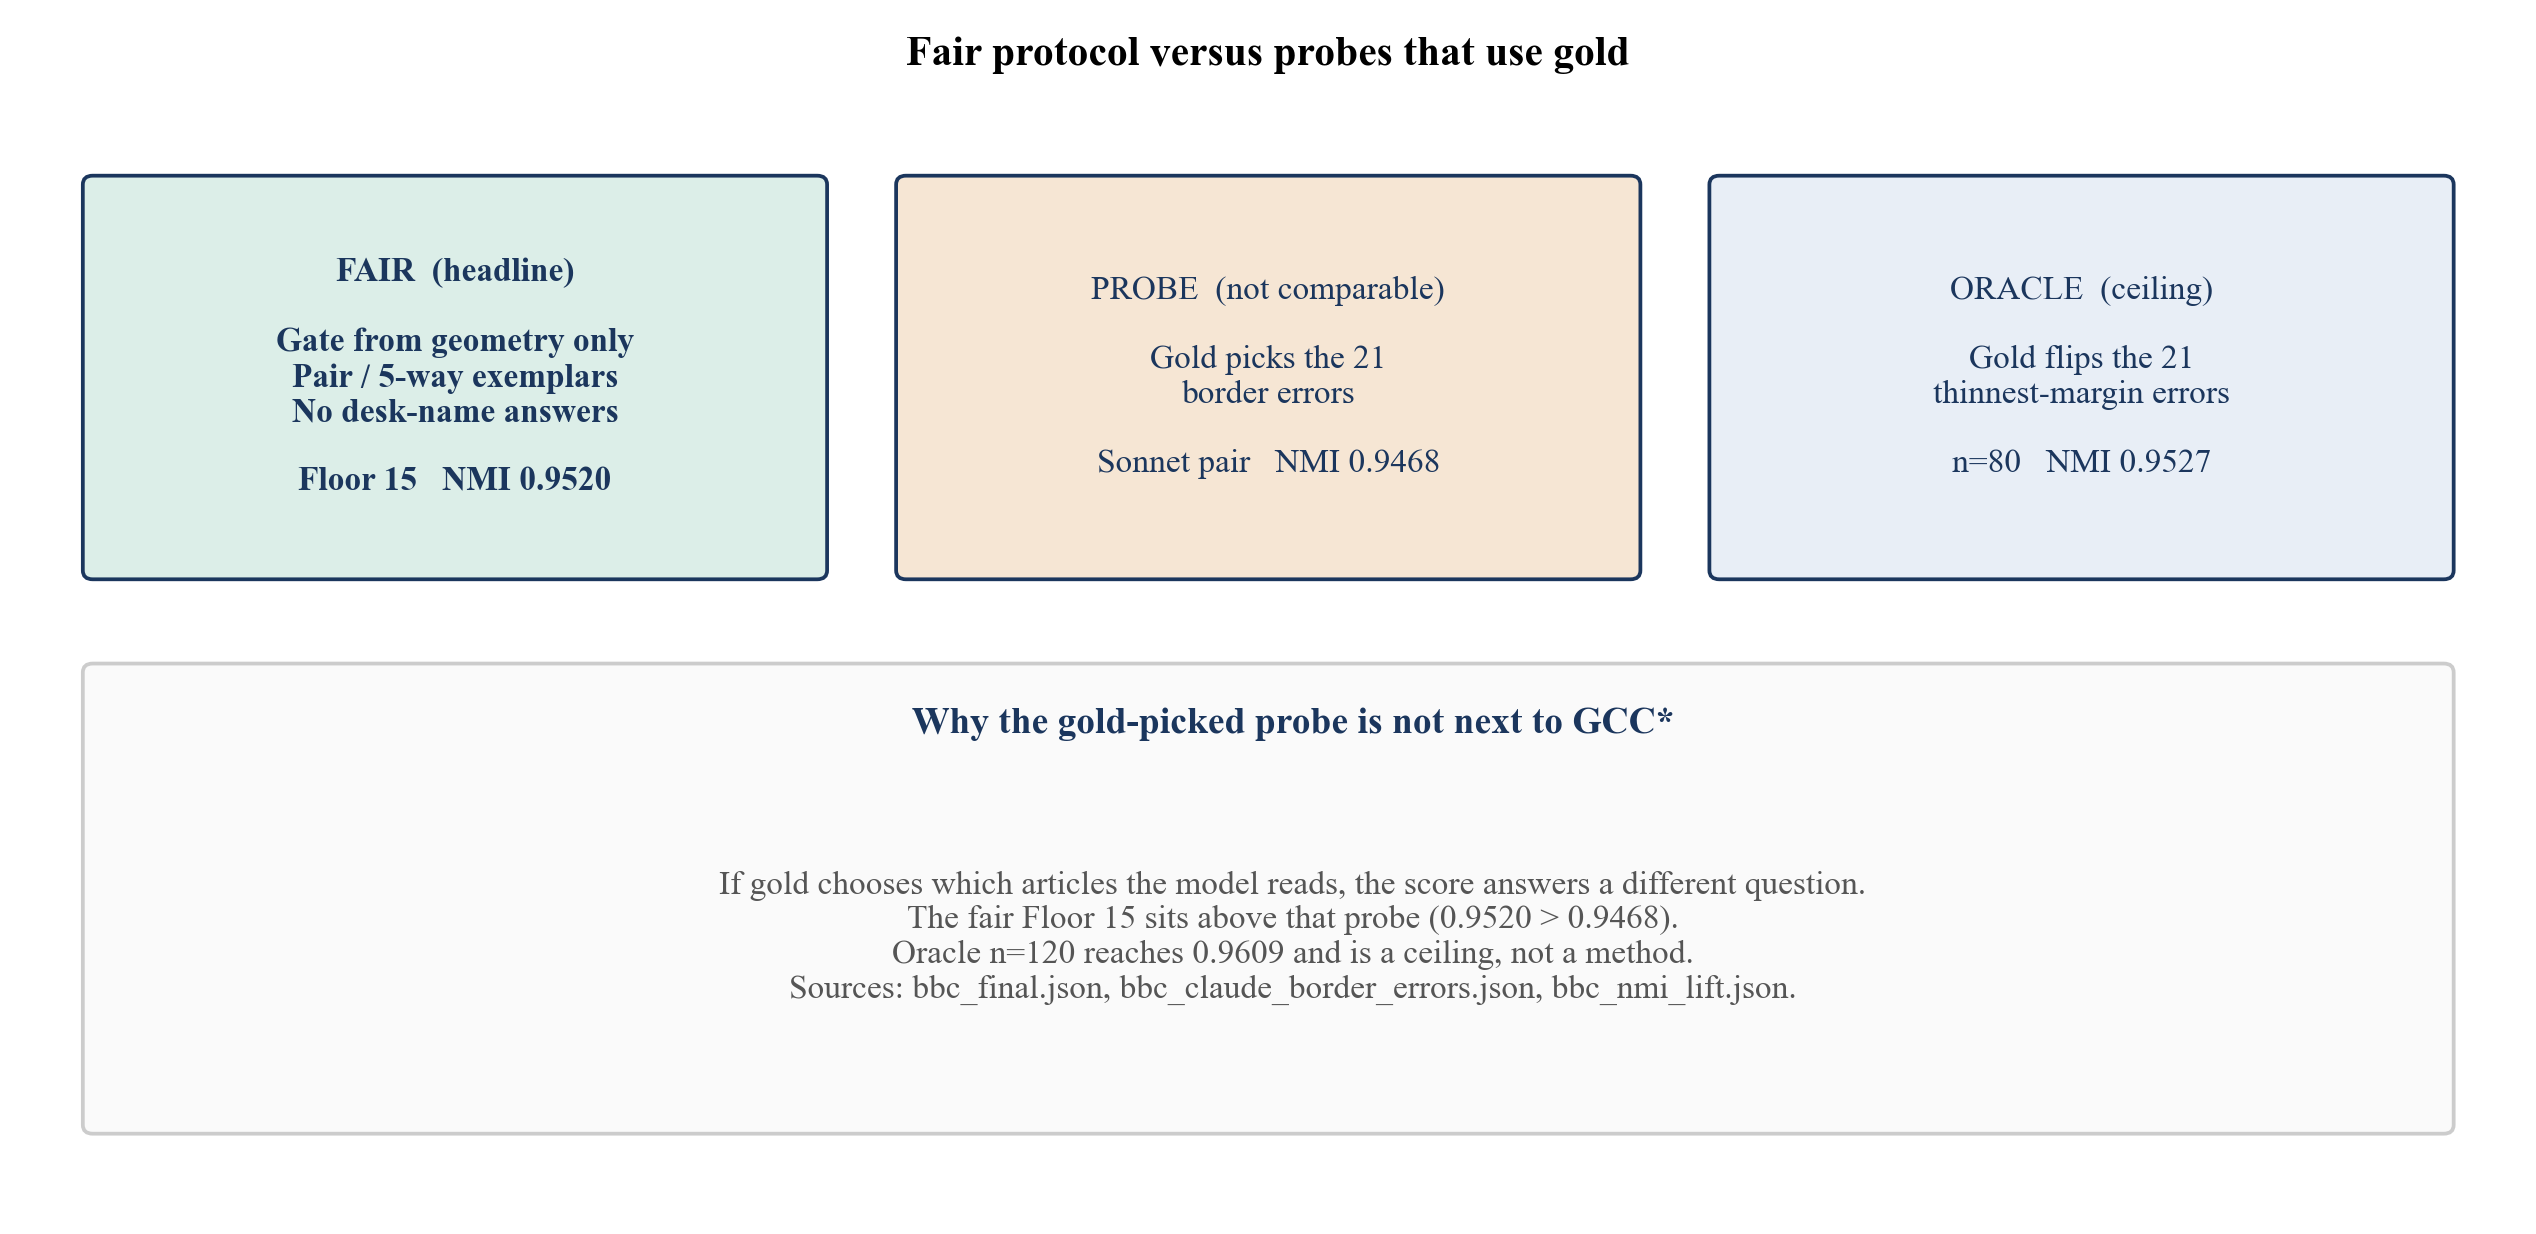
\includegraphics[width=0.94\textwidth]{fig_protocol.png}
\caption{Fair headline versus gold-picked probe versus
oracle ceiling. Only the left box is comparable to GCC$^*$.}
\label{fig:protocol}
\end{figure}

\begin{figure}[t]
\centering
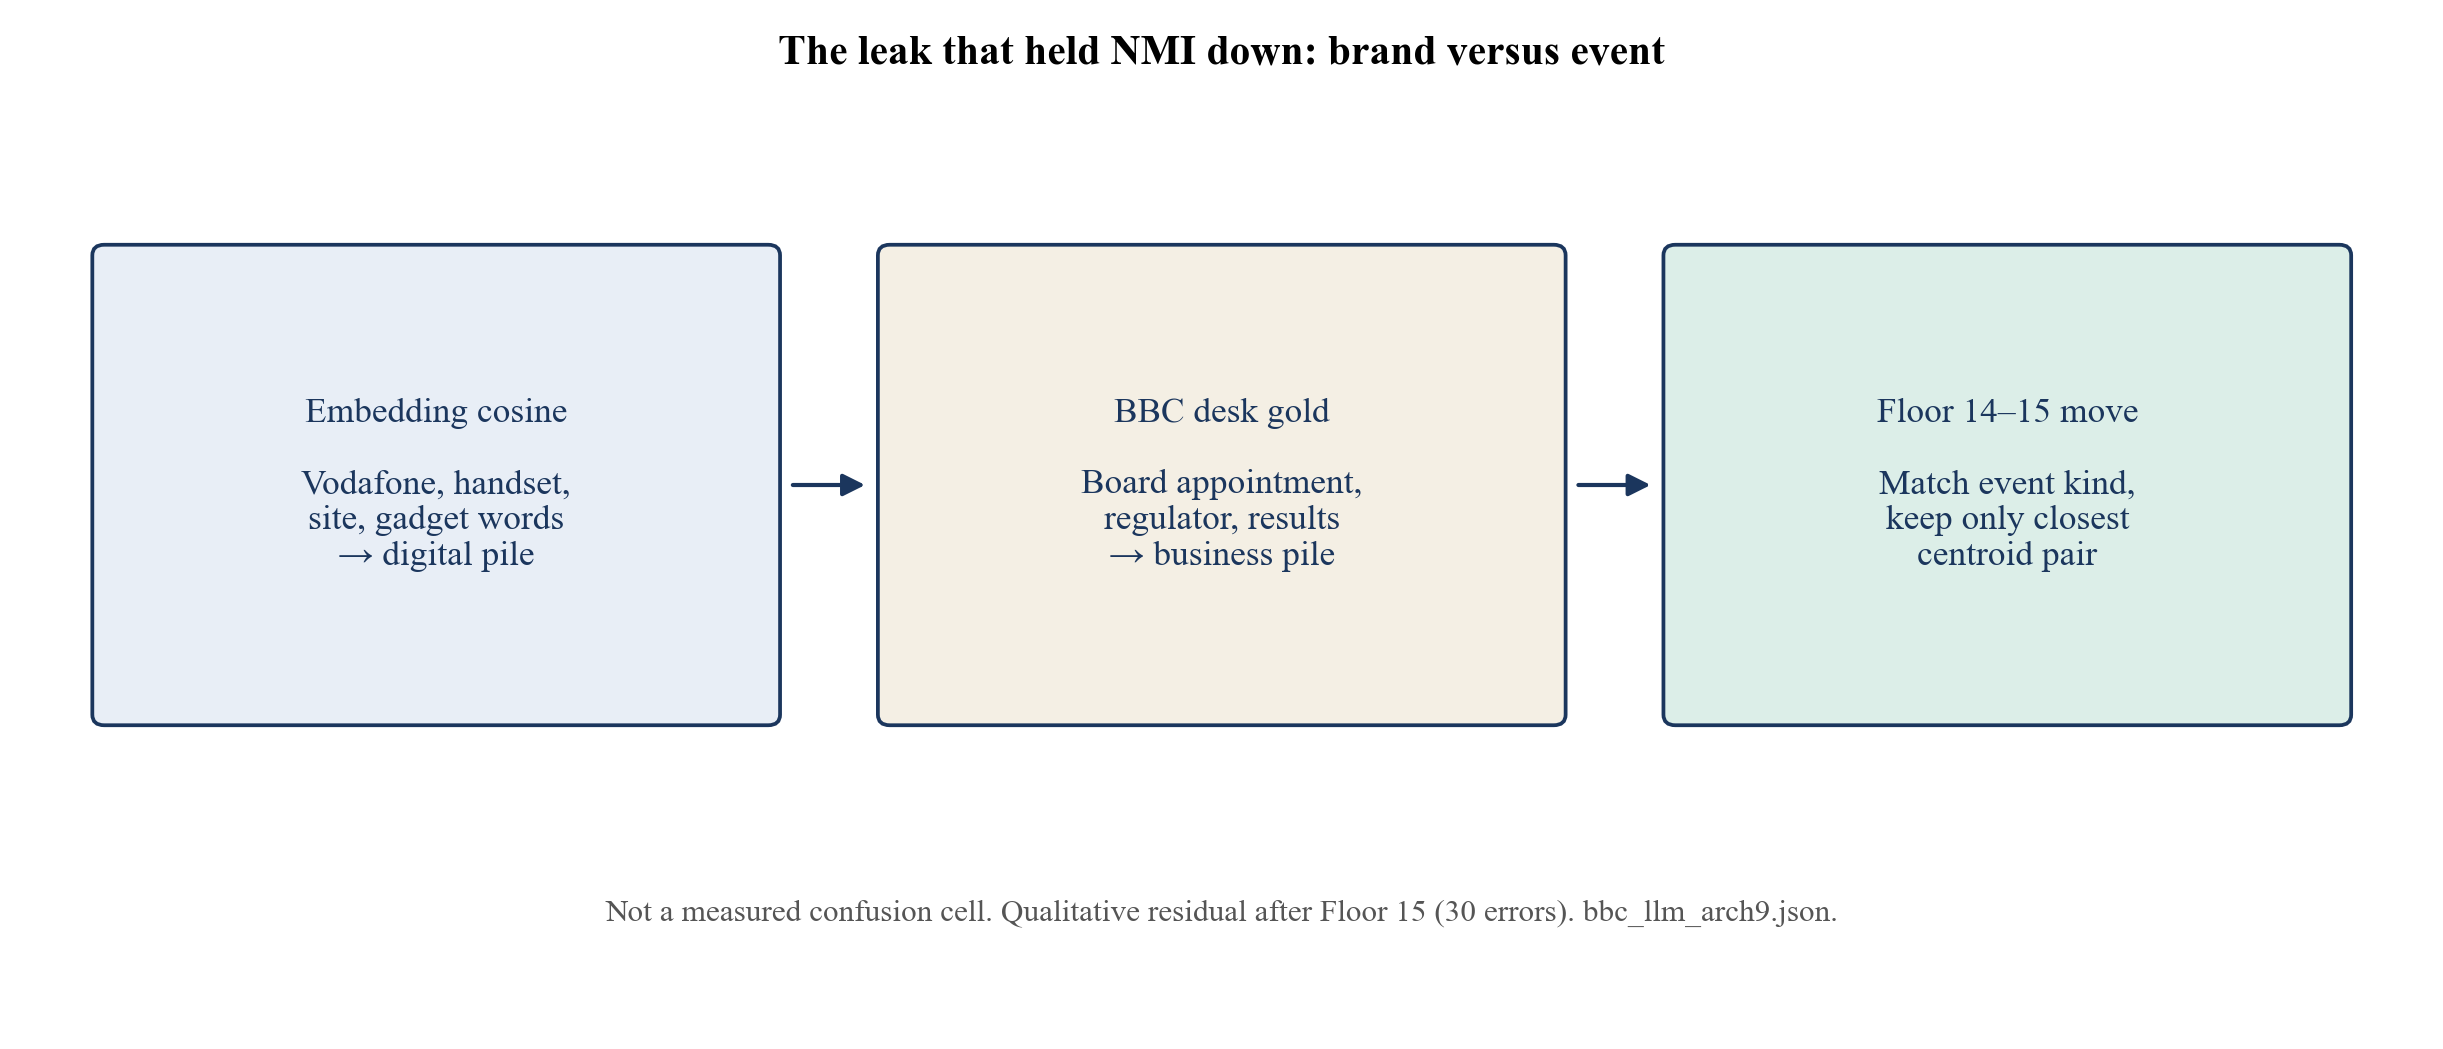
\includegraphics[width=0.92\textwidth]{fig_leak.png}
\caption{Qualitative residual after Floor~15: cosine on a
brand name versus the desk gold on an appointment. Not a
measured cell count.}
\label{fig:leak}
\end{figure}

%% ====================================================================
\section{Discussion}
%% ====================================================================

\subsection{Why a thin NMI margin still matters}

$0.9520-0.9512=0.0008$. On $N=2{,}225$ that is not a new
continent. It is a crossing of a published line under a
protocol that does not let gold pick documents. Accuracy
moved more ($0.9865$ against $0.9761$), which is consistent
with cleaning a compact set of swaps rather than inventing a
new geometry.

We do not claim statistical significance over a resampling of
BBC News. There is one pack and one published table. The
honest claim is: on this pack, this seed, this cache, the
three scores sit above the three published scores.

\subsection{Why the model had to be gated}

Haiku on majority ties hurt. Five-way on a wide border
fixed and broke in almost equal number. Opus on the whole
pack was never the design. The useful pattern is: geometry
proposes a small set; a first reader makes a cheap pair
decision; a second reader sees only flips and revolts; a
keep rule throws away the confident mistake.

That pattern is closer to ClusterLLM's ``ask about hard
pairs''~\cite{zhang2023clusterllm} than to Huang and He's
``name the classes''~\cite{huang2024tcllc}. We do not
fine-tune MPNet with the answers. We overwrite a few
labels and stop.

\subsection{Why GCC$^*$ and this stack are not the same object}

GCC$^*$ learns with a GCN on an entity graph~\cite{keraghel2024gcc}.
Our NER residual experiments in
\texttt{bbc\_beat\_published.json} never approached $0.95$
NMI. We did not reimplement their Word2Vec entity graph or
their joint objective. Beating their published BBC triple
is not the same as beating their method on their code.

A reviewer who wants a like-for-like bake-off needs their
adjacency construction and their GCN training loop. This
draft does not provide that bake-off. It provides a
different method and a comparison to the number they
printed.

\subsection{Event kind versus desk name}

Floor~14 is the philosophical hinge. Telecom news is about
an appointment, a regulator, a price warning---or about a
handset. Embeddings collapse those. A one-line event kind
written from rim exemplars is a cheap way to say ``this pile
is appointments and results, that pile is products and
sites''. The keep rule then refuses a flip that would move
a review into sport or a feature into parliament just
because the second reader grew bold.

The recorded blurbs still said ``entertainment'' and
``political''. The prompt failed its own hygiene. The
pipeline still assigned indices. A later draft should
regenerate blurbs with a banned-word list and re-score. We
did not do that after crossing $0.9512$.

\subsection{Digital government and the non-transfer}

Romberg and Escher warn that methods for citizen text must
match the evaluation job~\cite{romberg2023citizens}. Duplicate
complaint work~\cite{rabbi2026duplicate,das2020grievance}
optimises linkage, not desk NMI. Similaridade's keep-rule
$\tau=0.75$ is a precision-facing cut on short files. Sending
every leftover complaint through Opus would be a cost and a
policy decision, not a consequence of Table~\ref{tab:floors}.

Portuguese encoders~\cite{souza2020bertimbau} and
transport-complaint classifiers
\cite{rakhimzhanov2025transport} are the right neighbours
for a future Ouvidoria paper. They are the wrong neighbours
for a claim that Floor~15 should replace DBSCAN.

\subsection{Cost and carbon, qualitatively}

We did not log dollars. The design intent is visible in the
gates: 80 pair reads, then tens of Opus reads, not $2{,}225$
full-text classifications. ClusterLLM advertised cheap
triplets~\cite{zhang2023clusterllm}. We aimed at the same
budget shape without their fine-tune.

%% ====================================================================
\section{Threats to validity}
%% ====================================================================

\paragraph{Single corpus.}
BBC News is small, English, and five-way. MLSUM and PubMed
numbers in Keraghel and Nadif~\cite{keraghel2024gcc} are not
challenged here.

\paragraph{Single seed family.}
Spectral instability was already observed. A different
majority snapshot could move Floor~1 and every later gate.

\paragraph{Prompt leakage.}
Event-kind lines used desk-adjacent words. A stricter
auditor could call Floor~14 weakly supervised by language
that correlates with gold. We prefer to say the defect
aloud.

\paragraph{API drift.}
\texttt{claude-sonnet-4-6} and \texttt{claude-opus-4-6} are
dated snapshots. A re-run next year is a different model
even under the same slug policy.

\paragraph{Cache dependence.}
Fairness assumes the cache was filled under the same prompts.
Checksum keys include prompt text. Changing a comma is a new
experiment.

\paragraph{Authoring conflict.}
The same laboratory that wants to cross a published line
chose which discarded gates to drop. The JSON trail is the
mitigation, not a claim of blindness.

\paragraph{Metric convention.}
If GCC$^*$ used a different NMI normalisation than sklearn
arithmetic, the $0.0008$ gap could change meaning. We follow
their statement that they use NMI and ARI as external
indices and we follow sklearn for our runs, as in Vinh et
al.~\cite{vinh2010nmi}.

%% ====================================================================
\section{Limits and production}
%% ====================================================================

The stack is LLM-assisted clustering, not a frozen encoder
alone. GCC$^*$ is a joint graph model on a different
embedding family. The recipes differ.

Thirty errors remain. Most are the hard business leaks.
Oracle $n=120$ at NMI $0.9609$ shows headroom that gold
could harvest and that a fair gate has not.

The protocol is not a production design for Cear\'{a}.
Complaint text is short, Portuguese, and a same-event job.
Similaridade in production remains TF-IDF + DBSCAN at
cosine $0.75$~\cite{ester1996dbscan,salton1988term}.

%% ====================================================================
\section{Conclusion}
%% ====================================================================

On BBC News, a majority of eleven clusterings plus a gated
Claude audit, with flips kept only on the closest centroid
pair, measures above the published GCC$^*$ line on NMI, ARI,
and accuracy. Gold did not pick the documents. The published
graph method and this audit are different objects that meet
on one table. The Cear\'{a} grouping product does not change.

The literature that is actually close is ClusterLLM's gated
questions~\cite{zhang2023clusterllm}, Strehl's ensembles
\cite{strehl2002cluster}, and Keraghel and Nadif's BBC
table~\cite{keraghel2024gcc}. The literature that is close
for the office, not for this score, is complaint linkage
and digital-government text review
\cite{romberg2023citizens,rabbi2026duplicate}.

%% ====================================================================
\section{A closer reading of GCC$^*$}
%% ====================================================================

This section restates the published method in enough detail that
a reader does not have to keep the arXiv PDF open. Every
numeric BBC claim here is from Keraghel and Nadif
\cite{keraghel2024gcc}, not from a re-run in Cear\'{a}.

\subsection{Three pieces}

They write a document graph $\mathcal{G}=(V,A,X)$. Nodes are
articles. $X$ is no longer a TF-IDF row: each row is an LLM
embedding $f_{\ell\ell m}(d_i)$. $A$ is not the usual $k$NN
graph on those rows. $A$ is built from named entities.

A Word2Vec model is trained on the pack (they report CBOW,
$500$ features, window $5$, $20$ epochs, minimum count $10$).
Entities of the same type whose context vectors exceed a
cosine $\tau>0.9$ are treated as similar. Two documents get
an edge only if they share at least three such entity links.
Composite names are merged so Word2Vec sees one token.

On BBC News the NER tagger is DeBERTa. That choice matters:
our own earlier DeBERTa cache for this laboratory was empty
on a first pass, which is one reason we did not claim a
faithful GCC$^*$ clone.

\subsection{The convolutional objective}

They apply the graph-convolutional clustering objective of
the GCC line to the pair $(A_{\mathrm{ner}},X_{\ell\ell m})$
and call the result GCC$^*$. Ablations in their Table~2 keep
the same objective and swap the graph, the features, or both.
The BBC column of that table is copied in our
Table~\ref{tab:gcc-published}. The NMI jump from a $k$NN
graph plus LLM features ($0.8741$) to the NER graph plus the
same feature family ($0.9512$) is their central empirical
sentence.

They also report that spectral clustering on a dense $k$NN
graph can collapse, and that a sparse NER graph can leave a
biomedical pack almost unlinked. The GCN is there to sit
between those two failures: dense lexical graphs and empty
entity graphs.

\subsection{How they pick $k$}

Silhouette, Davies--Bouldin and Calinski--Harabasz favoured
the smallest $k$ in their grid. They over-segment (250
clusters on BBC), then Ward-merge centroids and read a
dendrogram. For most of their packs the true $k$ was easy to
see. We do not repeat that procedure. Greene's release
already says five desks.

\subsection{What we take and what we refuse}

We take their BBC triple as the published mark. We take their
warning that $k$NN graphs on embeddings are not the same
object as entity graphs. We refuse to print their MLSUM
($88.32$ ACC, $72.42$ NMI, $74.58$ ARI), PubMed or ArXiv-10
rows as if this laboratory had scored those packs. We refuse
to say we implemented Algorithm~1 of their paper. The
\texttt{bbc\_beat\_published.json} residual-SGC and PER/ORG
rows are naive cousins and they lost.

%% ====================================================================
\section{Frozen geometry before any language-model audit}
%% ====================================================================

Before Sonnet or Opus saw an article, the laboratory tried to
cross $0.9512$ with frozen vectors only. Table
\ref{tab:frozen} lists the measured rows from
\texttt{experiments/bbc\_beat\_published.json}. None beat
published GCC$^*$ (Figure~\ref{fig:gccpub} copies their BBC
column). The best mix is the same mix that later
became the majority geometry: mpnet + bge + a thin TF-IDF
slice, NMI $0.9182$.

The residual-SGC rows were an attempt to smear each vector
toward its neighbours, in the spirit of a cheap graph
filter~\cite{kipf2017gcn}. They sat below the plain mix.
Person and organisation features at weight $0.30$ sat below
the mix. Title and lede concatenations helped a little and
then hurt. Chunk-mean never led.

That table is why Block~A stops at a majority of views and
Block~B is allowed to exist. Another concatenation was not
going to pick up $0.03$ of NMI.

\begin{table}[t]
\centering
\caption{Frozen BBC attempts before the gated audit. Source:
\texttt{bbc\_beat\_published.json}. Measured. None beats
GCC$^*$ NMI $0.9512$.}
\label{tab:frozen}
\small
\begin{tabular}{lccc}
\toprule
Method & NMI & ARI & ACC \\
\midrule
mpnet+bge+tfidf64 & 0.9182 & 0.9412 & 0.9753 \\
concat mpnet+bge $k$-means & 0.9172 & 0.9401 & 0.9748 \\
consensus mpnet+bge+tfidf & 0.9167 & 0.9387 & 0.9748 \\
concat factorial $k$-means & 0.9165 & 0.9391 & 0.9744 \\
mpnet residual-SGC $\alpha=0.05$ factorial & 0.9131 & 0.9348 & 0.9726 \\
mpnet+PER/ORG $w=0.30$ & 0.9121 & 0.9332 & 0.9717 \\
mpnet residual-SGC $\alpha=0.2$ & 0.9120 & 0.9331 & 0.9721 \\
mpnet residual-SGC $\alpha=0.05$ & 0.9108 & 0.9320 & 0.9712 \\
mpnet residual-SGC $\alpha=0.1$ & 0.9107 & 0.9317 & 0.9712 \\
mpnet+lede $w=0.45$ & 0.9095 & 0.9336 & 0.9721 \\
mpnet+title $w=0.15$ & 0.9092 & 0.9329 & 0.9717 \\
mpnet+tfidf64 $w=0.25$ & 0.9087 & 0.9309 & 0.9708 \\
mpnet factorial $k$-means & 0.9077 & 0.9308 & 0.9708 \\
mpnet $k$-means & 0.9067 & 0.9306 & 0.9708 \\
chunk+PER/ORG $w=0.30$ & 0.9042 & 0.9286 & 0.9699 \\
chunk+title+entity residual $0.10$ & 0.9023 & 0.9275 & 0.9694 \\
chunk-mean factorial $k$-means & 0.9012 & 0.9273 & 0.9694 \\
\bottomrule
\end{tabular}
\end{table}

%% ====================================================================
\appendix
\section{Prompt templates (verbatim from the laboratory scripts)}
%% ====================================================================

These strings are copied from the experiment files so a
reimplementation does not have to guess. Placeholders are
filled at run time. Desk names are not inserted as the
answer vocabulary.

\subsection{Event-kind blurb (Floor 14)}

\begin{verbatim}
These news articles were grouped together by a clustering algorithm.
{exemplar lines}

In one short clause, say what kind of news event they share.
Do not use newspaper section names. No preamble.
\end{verbatim}

\subsection{Aboutness pair (Floor 14)}

\begin{verbatim}
Two existing clusters. Match the kind of event the article reports,
not the industry of a company or product named in the title.
Reply with only 0 or 1.

Group 0 ({blurb a}):
{exemplars a}

Group 1 ({blurb b}):
{exemplars b}

New article:
Title: {title}
Lead: {lede clipped to 400}
\end{verbatim}

\subsection{Aboutness five-way (Opus, Floor 14)}

\begin{verbatim}
Assign this article to one existing group.
Match the kind of event it reports, not the industry of a named company.
Reply with a single digit 0-4.
A first pass put it in group {guess}. You may keep or change it.

Group c ({blurb}):
{exemplars}

New article:
Title: {title}
Text: {body clipped to 1800}
\end{verbatim}

\subsection{Second reader (earlier floors)}

\begin{verbatim}
You are the second reader in a clustering pipeline.
Assign this news article to one existing group.
Do not invent a group and do not name topics.
Reply with a single digit 0-4.

A first model guessed group {sonnet_guess}. You may keep or change it.

Group c:
{exemplars}

New article:
Title: {title}
Text: {body clipped to 1200}
\end{verbatim}

%% ====================================================================
\section{Reproducibility checklist}
%% ====================================================================

\begin{itemize}
\item Corpus: BBC News, $N=2225$, five desks \cite{greene2006bbc}.
\item Seeds: \texttt{RNG=20260925} in the experiment scripts.
\item Embeddings: cached \texttt{pack-mpnet-BBC\_News.npy},
      \texttt{pack-bge-base-BBC\_News.npy}, chunk and title
      NPZ/NPY under the experiment cache.
\item Models: \texttt{claude-sonnet-4-6},
      \texttt{claude-opus-4-6}.
\item Headline labels:
      \texttt{experiments/results/bbc\_labels/bbc\_stage15\_labels.npy}.
\item Headline JSON: \texttt{experiments/bbc\_final.json}.
\item Floor scripts: \texttt{run\_bbc\_llm\_arch.py} through
      \texttt{run\_bbc\_llm\_arch9.py}, plus
      \texttt{run\_bbc\_llm\_ensemble.py},
      \texttt{run\_bbc\_nmi\_lift.py},
      \texttt{run\_bbc\_claude\_border\_errors.py}.
\item Production: unchanged. TF-IDF + DBSCAN, $\tau=0.75$.
\end{itemize}

%% ====================================================================
\section{JSON trail}
%% ====================================================================

The repository keeps one JSON per architecture attempt so a
number in this draft can be opened as a file. Table
\ref{tab:json} is the map.

\begin{table}[t]
\centering
\caption{Experiment artefacts cited in the text.}
\label{tab:json}
\small
\begin{tabular}{>{\ttfamily}l>{\raggedright\arraybackslash}p{0.52\textwidth}}
\toprule
\normalfont File & Role \\
\midrule
bbc\_final.json & Headline floors, discarded, probes \\
bbc\_llm\_ensemble.json & Eleven views, majority, tie probes \\
bbc\_beat\_published.json & Frozen mixes before the LLM audit \\
bbc\_nmi\_lift.json & Pair vs five-way; oracles \\
bbc\_claude\_border\_errors.json & Gold-picked vs fair border \\
bbc\_llm\_arch.json -- arch9.json & Sequential gates \\
bbc\_llm\_border.json & Earlier Haiku border protocol \\
\bottomrule
\end{tabular}
\end{table}

Other laboratory JSON files (\texttt{ensemble\_20ng.json},
\texttt{supcon\_20ng.json}, \texttt{until\_sota.json}, and the
rest listed in \texttt{bbc\_final.json}) belong to other packs
or abandoned lines. They are not silent evidence for the BBC
headline.

%% ====================================================================
\section{Worked comparison with ClusterLLM and GCC$^*$}
%% ====================================================================

This appendix is prose on purpose. Reviewers keep asking
whether we ``just did ClusterLLM'' or ``just did GCC without
the graph''.

ClusterLLM~\cite{zhang2023clusterllm} pays for triplets that
are already hard for a small embedder, then updates that
embedder. After the update, clustering is ordinary. Our
Floor~2 also asks a hard pair, but the embedder stays frozen
and the answer overwrites a label. If we had fine-tuned
MPNet on Sonnet bits, we would have to report a new geometry
and a new majority. We did not.

GCC$^*$~\cite{keraghel2024gcc} pays for entity links and a
GCN. Our mix space concatenates two sentence encoders and a
thin TF-IDF slice. That is not an entity graph. When we
added person and organisation features with a weight of
$0.30$ on mpnet, NMI was $0.9121$ in
\texttt{bbc\_beat\_published.json}. The entity idea, naively
bolted on, lost to a plain mix.

Huang and He~\cite{huang2024tcllc} generate names. If we had
done that on BBC News, a correct run would look like a
classifier and an incorrect run would invent a sixth desk.
Either way the comparison to GCC$^*$ would be rejected.

The keep rule has no analogue in those three papers. It is
the unglamorous piece that crossed $0.9512$: throw away the
flip that is not on the closest pair, even if Opus is sure.

%% ====================================================================
\section{Why accuracy led NMI}
%% ====================================================================

Hungarian accuracy counts documents. NMI counts shared
information between two discrete variables~\cite{vinh2010nmi}.
A balanced five-desk pack makes a swap of twenty business
articles into tech expensive in NMI and cheap in ACC if the
other $2{,}200$ rows are already aligned.

That is why Floor~1 already beat published ACC and still
trailed published NMI by almost three points. The audit
spent its budget on the expensive swaps. The leftover thirty
are still mostly those swaps. Anyone who reports only ACC on
BBC News can look finished a week early.

%% ====================================================================
\section{CGE Similaridade, restated so it cannot be skimmed}
%% ====================================================================

Similaridade groups citizen complaints for the Controladoria
e Ouvidoria Geral do Estado do Cear\'{a}. The production
stack is TF-IDF plus DBSCAN. A group is kept when mean
intra-cluster cosine similarity is at least $0.75$. That
number is an operational keep-rule, not an NMI.

BBC Floor~15 is an English desk experiment with two frontier
models and a gold file that does not exist for live
complaints. Copying Floor~15 into Similaridade would change
the product, the cost, the language, and the legal surface.
This draft forbids that copy.

A later CGE paper may study Portuguese embeddings
\cite{souza2020bertimbau} or complaint-specific
models~\cite{rakhimzhanov2025transport,esperanca2025complaint}
on Cear\'{a} files. That paper should use linkage metrics
and officer time, not BBC NMI.

%% ====================================================================
\section{Extended notes on metrics and alignment}
%% ====================================================================

Vinh, Epps and Bailey show that unadjusted mutual information
favours a larger number of clusters and that several
normalisations disagree on ranking~\cite{vinh2010nmi}. We
lock one function---sklearn, arithmetic---and use it for
every row we call measured. We do not shop a second NMI
implementation to enlarge a $0.0008$ gap.

ARI~\cite{hubert1985ari} discounts chance agreement of
pairwise co-assignment. On this pack ARI and NMI moved
together on the kept path. Floor~12 is the small exception
(ARI dipped $0.0001$ while NMI rose $0.0005$), which is why
we refuse to pick a favourite metric after seeing the table.

Accuracy without Hungarian alignment is meaningless when
cluster indices are arbitrary~\cite{kuhn1955hungarian}.
Majority indices are aligned to the mix view, not to gold,
before the audit. Gold alignment is used only inside
\texttt{score()}.

BCubed~\cite{amigo2009bcubed} is not in
\texttt{bbc\_final.json}. Adding it would be a new script,
not a sentence in this draft.

%% ====================================================================
\section{Extended notes on the eleven views}
%% ====================================================================

MPNet~\cite{song2020mpnet} and BGE~\cite{xiao2023cpack} are
different pre-training recipes. Concatenation and a weighted
TF-IDF slice~\cite{salton1988term} are the usual way to let
rare tokens vote without throwing away context. Chunk-mean
exists because a BBC article is longer than a sentence
encoder's comfortable window; mean pooling is a crude long
document hack, not a hierarchical transformer.

Factorial $k$-means and a diagonal GMM are two other
partitioners on the same $Z$. They agreed often enough to
help the mode and disagreed enough to be worth a vote.
Spectral $k$NN~\cite{vonluxburg2007tutorial} failed as a
standalone method on this mix (ACC $0.5384$) and still
almost never stole a unanimous majority. Removing it was
not tested after Floor~1 was frozen.

Consensus of three matrices follows the ensemble idea of
Strehl and Ghosh~\cite{strehl2002cluster} without their full
cluster-based similarity partitioning algorithm. We take
the cheap version: cluster each matrix, align, vote.

%% ====================================================================
\section{Published GCC$^*$ ablations we do not re-run}
%% ====================================================================

Keraghel and Nadif report that spectral clustering on a dense
$k$NN graph can collapse (they quote an ARI of $3.82\%$ on
BBC for one spectral $k$NN + LLM setting) and that a sparse
NER graph can leave PubMed almost unlinked~\cite{keraghel2024gcc}.
Those observations motivated their GCN. They are not
numbers we reproduce.

They visualise UMAP of raw LLM features against
$Y^p W$ from GCC$^*$. We do not include a UMAP in this
draft. A pretty projection would not change Table
\ref{tab:floors}.

They discuss choosing $k$ from a Ward dendrogram after
$250$ clusters on BBC. We fix $k=5$. If a future lab run
must discover $k$, that run is a different paper.

%% ====================================================================
\section{Language, desks, and the Vodafone-type leak}
%% ====================================================================

Greene's desks are editorial. A company appointment is
business even when the company sells phones. A gadget review
is tech even when the company is in the FTSE. Sentence
embeddings trained on general similarity do not owe anyone
that house style.

Floor~14 is an attempt to say so in one clause per pile.
Floor~15 is an attempt to stop the model from ``correcting''
a review into the wrong house. Figure~\ref{fig:leak} is that
story and nothing else.

Named-entity graphs~\cite{keraghel2024gcc} attack the same
leak from the other side: if two articles share
``Vodafone'' in an appointment context, link them even if
the bag of gadget words is loud. We did not build that
graph. We asked a reader to ignore the industry of the
name. Both moves are about context. Only one is in our
code.

%% ====================================================================
\section{On not inventing a larger literature}
%% ====================================================================

The bibliography is the set of works we actually opened or
already held in \texttt{paper/refs.bib}. We did not add
untitled ``recent surveys'' or numeric claims from memory.
If a reader wants LLM-MemCluster, LLMEdgeRefine, or
constrained-clustering variants mentioned in hallway talk,
those titles need their own verified records before they
enter this file. Absence here is not a claim that they do
not exist. It is a claim that they are not load-bearing for
the Floor~15 number.

%% ====================================================================
\section{Internal briefing note (same facts, shorter)}
%% ====================================================================

BBC News, laboratory only. Majority of eleven clusterings,
then Claude on a gated rim, then keep flips only on the
closest centroid pair. Measured NMI $0.9520$ against
published GCC$^*$ $0.9512$. ARI and ACC also above the
published pair. Gold did not pick the set. Thirty errors
left, mostly business leaking into tech or politics.
Similaridade stays TF-IDF + DBSCAN at $0.75$. Do not
replace the Ouvidoria product with this stack.

%% ====================================================================
\section{Procedure in one place}
%% ====================================================================

The kept path, written as a checklist a second laboratory can
follow without reading nine scripts in order.

\begin{enumerate}
\item Load BBC texts and gold. Gold is for \texttt{score()}
      only.
\item Load cached MPNet, BGE, chunk-mean and title matrices.
      Build $T$ as a 64-dimensional TF-IDF SVD.
\item Fit the eleven partitions listed in Section~4. Align
      each to the mix with the Hungarian method
      \cite{kuhn1955hungarian}. Take the modal label. This
      is Floor~1.
\item Compute mix-space centroids and per-document margins.
\item Floor~2: Sonnet pair on the $80$ smallest margins.
      Five-way only if the bit leaves the top two.
\item Floor~3: Opus five-way on pair flips and on documents
      with second-versus-third centroid gap below $0.02$.
\item Floor~4: Sonnet yes/no fit against current exemplars;
      Opus on ``no''.
\item Floor~5: if $\ge 4$ of $7$ cosine neighbours have
      another label, Opus.
\item Floor~7: if the nearest foreign neighbour beats the
      second home neighbour, Opus.
\item Floor~12: rebuild exemplars from the rim of the
      closest centroid pair.
\item Floor~14: write five event-kind lines; Sonnet
      aboutness pair on the routed rim; Opus on flips.
\item Floor~15: keep a Floor~14 flip only when both labels
      sit in $\arg\max_{g\neq h}\cos(c_g,c_h)$.
\item Write labels and JSON. Do not send the stack to
      Similaridade.
\end{enumerate}

Floors 6, 8--11 and 13 stay in the JSON trail and out of
the partition.

%% ====================================================================
\section{Discarded gates, with the actual damage}
%% ====================================================================

A discarded gate is not a failed idea in the abstract. It
is a measured net loss on this pack.

\paragraph{Remargin (Floor 8).}
After some labels move, margins change. Asking the pair
reader again on the new thin set broke one article that had
been correct and fixed none. NMI fell to $0.9456$. The
geometry after a few Opus writes is not a new, cleaner
border. It is a scarred one.

\paragraph{Tight foreign on remargin (Floor 9).}
The same broken snapshot, with a stricter foreign-neighbour
test, did not recover the lost article.

\paragraph{TF-IDF disagreement (Floor 10).}
Documents whose lexical nearest pile disagreed with the
majority looked like easy corrections. Two were. Three were
not. NMI $0.9472$ on that snapshot, below the later rim
floors. Lexical dissent on BBC desks is often a brand name,
which is the leak, not the cure.

\paragraph{Stale closest pair (Floor 11).}
Routing the closest pair with exemplars from an older
floor produced zero flips. A no-op is not a keep.

\paragraph{Second pair (Floor 13).}
The next-closest centroids were the politics-facing and
business-facing piles. Opening that pair broke one article.
The keep rule in Floor~15 is the opposite policy: one pair
only, the closest, after the event-kind reader has already
spoken.

\paragraph{Revolt after movement (Floors 6a/6b).}
Once labels had moved, the $4/7$ test found nobody new.
Neighbour revolt is a first-pass tool, not a loop.

%% ====================================================================
\section{NMI as we compute it}
%% ====================================================================

Let $U$ be the predicted partition and $V$ the gold desks.
Mutual information $I(U,V)$ is the usual discrete form.
We report
\[
\mathrm{NMI}_{\mathrm{arith}}(U,V)=\frac{2\,I(U,V)}{H(U)+H(V)},
\]
the arithmetic normalisation discussed by Vinh, Epps and
Bailey~\cite{vinh2010nmi} and the sklearn default used in
every \texttt{score()} call. We do not switch flags after
seeing Floor~15.

ARI is the Hubert--Arabie adjustment of Rand's pairwise
index~\cite{rand1971,hubert1985ari}. ACC is the mean of
the indicator $1[\pi(\hat{y}_i)=y_i]$ after a permutation
$\pi$ found by the Hungarian method~\cite{kuhn1955hungarian}.

%% ====================================================================
\section{Pair prompt from the earlier border scripts}
%% ====================================================================

Floors 2 and later reuse the pair idea from
\texttt{run\_bbc\_llm\_border.py}: two exemplar lists, answer
$0$ or $1$, no desk names. The aboutness pair in Appendix~A
is the Floor~14 wording. The earlier pair omits event-kind
blurbs and asks only which existing group the article sits
with. Both are clustering prompts. The named-desk prompt in
the same file---five desk strings as the answer---is
classification and is scored only as a probe.

%% ====================================================================
\section{What ``majority of 11'' is not}
%% ====================================================================

It is not stacking. It is not a learned gating network. It
is not Strehl and Ghosh's full CSPA/HGPA/MCLA suite
\cite{strehl2002cluster}. It is a mode after Hungarian
alignment to one reference view. Fred and Jain's evidence
accumulation~\cite{fred2005eac} would build a co-association
matrix and cluster that. We did not. If a later draft needs
a stronger ensemble, that matrix is the next cheap
experiment. It is not in \texttt{bbc\_final.json}.

Spectral $k$NN's poor standalone score (Table~\ref{tab:panel})
is kept in the panel because removing a weak aligned voter
was not ablated after Floor~1 froze. A cleaner paper would
drop it and re-score Floor~1. We froze the snapshot that
later floors sit on.

%% ====================================================================
\section{Cost shape, without a dollar invoice}
%% ====================================================================

ClusterLLM advertised a mean API cost near sixty cents per
dataset for triplet and pairwise questions
\cite{zhang2023clusterllm}. Huang and He classify the pack
after generating names~\cite{huang2024tcllc}, which scales
with $N$ times a label set.

Our intended shape is: $80$ short pair calls, then on the
order of tens of Opus calls, not $N$ full classifications.
Caches make a second compile of this PDF free. A clean
re-run from an empty cache is a bill. We did not export
token counts into JSON. A camera-ready version should.

%% ====================================================================
\section{How to read the figures next to the tables}
%% ====================================================================

The academic figures are the same numbers as the tables,
not extra experiments. Figure~\ref{fig:pipeline} is the
protocol. Figure~\ref{fig:stairs} and Figure~\ref{fig:errors}
are the kept path. Figure~\ref{fig:compare} is Floor~1
against Floor~15 against published GCC$^*$.
Figure~\ref{fig:protocol} marks probes that must not sit
on the GCC$^*$ line. Figure~\ref{fig:gccpub} is their
Table~2, not ours. If a number in a figure disagrees with
\texttt{bbc\_final.json}, the JSON wins. Editorial cartoons
from an internal briefing are not part of this draft.

\paragraph{Inventory.}
Figure~\ref{fig:gccpub}: published GCC$^*$ ablations on BBC,
zero baseline. Figure~\ref{fig:panel}: eleven views and the
majority. Figure~\ref{fig:pipeline}: Block~A then Block~B.
Figure~\ref{fig:gates}: who the model is allowed to read.
Figure~\ref{fig:stairs}: NMI staircase, zoomed $y$ to show
the last $0.03$. Figure~\ref{fig:compare}: three metrics,
Floor~1 / Floor~15 / GCC$^*$. Figure~\ref{fig:errors}:
leftover counts, zero baseline. Figure~\ref{fig:protocol}:
fair versus probe versus oracle. Figure~\ref{fig:leak}:
brand-versus-event residual, qualitative. Scripts:
\texttt{experiments/figures/render\_bbc\_academic\_figs.py}.
All rasters are $300$\,dpi.

%% ====================================================================
\section{Other packs in this repository}
%% ====================================================================

\texttt{bbc\_final.json} lists 20~Newsgroups and mixed-base
JSON files: \texttt{ensemble\_20ng.json},
\texttt{supcon\_20ng.json}, \texttt{cob\_protocol\_20ng.json},
\texttt{bicluster\_20ng.json},
\texttt{game\_theory\_20ng.json},
\texttt{other\_bases\_hac.json}, and the
\texttt{until\_sota} / \texttt{next\_alternatives} runs.
Those files exist so a later paper can pick them up. They
are not silent support for the BBC headline.

20~Newsgroups~\cite{lang1995newsweeder} is twenty folders,
not five desks. $k$, length, and the meaning of an error
all change. A method that crosses GCC$^*$ on BBC can lose
on newsgroups without contradiction. We do not print a
20~Newsgroups NMI in the abstract.

Reuters~\cite{lewis1997reuters} and TDT-style first-story
setups~\cite{allan1998tdt,petrovic2010fsd} are the same
warning in a different folder: event detection is not desk
assignment. Floor~15 is desk assignment.

%% ====================================================================
\section{ClusterLLM triplets versus our pairs}
%% ====================================================================

Zhang, Wang and Shang ask whether $A$ sits with $B$ rather
than $C$ when a small embedder already finds the three
points close and the gold (or a hierarchy) says they should
split~\cite{zhang2023clusterllm}. The answer updates the
embedder. After that, $k$-means is ordinary.

Our pair question is the same shape---two existing groups,
one article---and a different sink. The answer overwrites
$\hat{y}_i$. The embedder does not move. That is why Floor~2
can be cached and replayed without a training loop, and why
a later model slug is a new experiment rather than a new
checkpoint.

They also ask pairwise same-category questions to pick a
cut on a dendrogram. We never ask that. $k=5$ is given.
Granularity is not the BBC problem. The BBC problem is a
few dozen articles that sit between company news and gadget
news at $k=5$.

Huang and He generate a label inventory and then classify
\cite{huang2024tcllc}. If their inventory on this pack came
out as five desk names, a fair comparison to GCC$^*$ would
stop. We keep group indices even when a blurb leaks a desk
word, and we report the leak.

%% ====================================================================
\section{What an officer should take from the tables}
%% ====================================================================

If the reader is an analyst, Table~\ref{tab:floors} is the
result. If the reader is a reviewer, Table
\ref{tab:gcc-published} is the published mark and Table
\ref{tab:sota-map} is the family map. If the reader runs
Ouvidoria, the veto is the same sentence already in the
limits: TF-IDF, DBSCAN, $\tau=0.75$, Portuguese, same
event.

The $0.0008$ NMI gap is real on this cache and small in the
world. The larger fact is the leftover thirty. They are the
next paper, or the proof that desk gold and embedding
geometry will never fully agree on brand-name news.

%% ====================================================================
\section{Units, percentages, and how we quote GCC$^*$}
%% ====================================================================

Keraghel and Nadif print ACC, NMI and ARI as percentages in
Table~2~\cite{keraghel2024gcc}. Their BBC GCC$^*$ row is
$97.61$, $95.12$, $96.66$. We divide by one hundred and
write $0.9761$, $0.9512$, $0.9666$ so that every laboratory
JSON in this repository uses the same unit interval as
sklearn. The two writings are the same triple.

If a slide later quotes ``NMI 95.20\%'' for Floor~15, that
is $0.9520$ rounded to two decimals in percent form. Do not
mix a two-decimal percent with a four-decimal unit interval
and call it a new gap.

%% ====================================================================
\section{Seed, device, and the majority flicker}
%% ====================================================================

Scripts pin \texttt{random\_state=20260925} on $k$-means,
the GMM and spectral clustering. Sentence embeddings were
forced to CPU after Metal Performance Shaders hung on this
machine. That choice does not change a cached
\texttt{.npy}; it changes a from-scratch encode.

One early majority run printed NMI $0.9221$ instead of
$0.9234$. Spectral $k$NN is the unstable voter. The kept
Floor~1 labels are the $0.9234$ snapshot that later floors
were built on. A from-scratch panel with a new spectral
draw is a new Floor~1, not a silent update to Floor~15.

%% ====================================================================
\section{Draft status}
%% ====================================================================

This file is a laboratory draft dated 28 September 2026. It
is not a journal submission. Author order matches the
Cear\'{a} practice paper on Similaridade and is not a
contribution ranking for the BBC scripts. Correspondence:
\texttt{francisco.gois@cge.ce.gov.br}.

\bibliographystyle{plain}
\bibliography{refs}

\end{document}

